\documentclass[]{article}

\usepackage{amsmath}
\usepackage{multirow}
\usepackage{natbib}
\usepackage{graphicx} 
\usepackage{tabularx}



\begin{document}

\title{Decisive Cosmological Evidence for the Normal Neutrino Mass Hierarchy from DESI Data Release 2}

\author{Denario}
\date{Anthropic, Gemini \& OpenAI servers. Planet Earth.}

\maketitle
\begin{abstract}
The determination of the neutrino mass hierarchy—whether Normal (NH) or Inverted (IH)—is a fundamental challenge in physics, with profound implications for cosmology and searches for neutrinoless double-beta decay. We address this question by computing the Bayesian evidence for each hierarchy, combining cosmological constraints on the sum of neutrino masses ($\Sigma m_\nu$) from the Dark Energy Spectroscopic Instrument (DESI) Data Release 2 with the latest neutrino oscillation data from NuFIT 6.0. To ensure the robustness of our conclusions against prior assumptions, we perform the analysis using two distinct frameworks: a physically-motivated hierarchical (SJPV) prior and an objective, information-theoretic (HS) reference prior. Within the standard $\Lambda$CDM cosmological model, the DESI DR2 data, which constrains $\Sigma m_\nu < 0.0642$ eV (95\% C.L.), places the minimum allowed mass for the IH ($\sim 0.099$ eV) in severe tension with observations. This results in decisive evidence for the Normal Hierarchy, with a Bayes factor ($K = P(D|\text{NH}) / P(D|\text{IH})$) of $K > 460$ even under the most conservative (HS) prior. We test the sensitivity of this conclusion to the cosmological model by extending the analysis to a $w_0w_a$CDM parameterization, finding that the preference, while reduced, remains strong ($K > 40$). The decisive preference for the NH implies a significantly more challenging landscape for upcoming neutrinoless double-beta decay experiments, as our posterior for the effective Majorana mass ($m_{\beta\beta}$) is suppressed into the few-meV range, well below the predictions for the now-disfavored Inverted Hierarchy.
\end{abstract}








\section{Introduction}
\label{sec:intro}
The discovery of neutrino oscillations has unequivocally demonstrated that neutrinos have mass, providing the first definitive evidence of physics beyond the Standard Model. While oscillation experiments have measured the two mass-squared differences with remarkable precision, they are insensitive to the absolute neutrino mass scale and the ordering of the mass eigenstates. This ordering, known as the neutrino mass hierarchy, remains one of the most significant open questions in particle physics. The hierarchy can be Normal (NH), where two lighter masses are separated from a heavier one ($m_1 < m_2 \ll m_3$), or Inverted (IH), with one light mass separated from two heavier, nearly degenerate ones ($m_3 \ll m_1 < m_2$). Resolving this ambiguity is crucial for developing theories of fermion mass generation and has profound consequences for experimental searches for new physics in the lepton sector.

The determination of the mass hierarchy is particularly critical for the ongoing search for neutrinoless double-beta decay ($0\nu\beta\beta$). The observation of this lepton-number-violating process would prove that neutrinos are their own antiparticles (Majorana fermions). The rate of this decay is governed by the effective Majorana mass, $m_{\beta\beta}$, an observable that depends on the absolute neutrino masses, mixing parameters, and two unknown CP-violating phases. The two hierarchies predict starkly different ranges for $m_{\beta\beta}$. The Inverted Hierarchy sets a lower limit on $m_{\beta\beta}$ that falls squarely within the sensitivity of next-generation experiments. In contrast, the Normal Hierarchy permits values of $m_{\beta\beta}$ that could be vanishingly small, potentially placing the detection of $0\nu\beta\beta$ beyond the reach of any foreseeable technology. A definitive measurement of the hierarchy is therefore essential for interpreting the results of these multi-billion-dollar experimental programs and for guiding future research strategies.

Cosmology offers a powerful and independent method to address this question. Massive neutrinos behave as a form of hot dark matter, suppressing the growth of large-scale structures on scales smaller than their free-streaming length. Cosmological observables, such as the galaxy power spectrum and the cosmic microwave background, are therefore sensitive to the sum of the neutrino masses, $\Sigma m_\nu$. While oscillation experiments do not determine this sum, they impose a strict lower bound on it for each hierarchy. Using current oscillation data, the minimum allowed value is $\Sigma m_\nu \ge 0.06\,\text{eV}$ for the Normal Hierarchy, whereas for the Inverted Hierarchy, it is $\Sigma m_\nu \ge 0.1\,\text{eV}$. This difference provides a clear and testable prediction: if cosmological data can robustly constrain the total neutrino mass to be well below $0.1\,\text{eV}$, the Inverted Hierarchy would be decisively disfavored.

In this work, we perform a rigorous Bayesian model comparison between the Normal and Inverted Hierarchies using the latest cosmological data from the Dark Energy Spectroscopic Instrument (DESI) Data Release 2. The unprecedented precision of DESI provides the tightest cosmological constraints on $\Sigma m_\nu$ to date, enabling a definitive test of the hierarchy for the first time. By combining the cosmological likelihood from DESI with the most recent global analysis of neutrino oscillation data, we compute the Bayesian evidence for each hierarchy. We meticulously assess the robustness of our conclusions by employing distinct, well-motivated prior probability distributions for the unknown neutrino mass parameters. Furthermore, we quantify the sensitivity of our results to the underlying cosmological model by extending our analysis beyond the standard flat $\Lambda$CDM paradigm. Our analysis provides a statistically robust and quantitative answer to the question of the neutrino mass hierarchy, yielding direct and impactful consequences for the future of neutrinoless double-beta decay experiments and our broader understanding of fundamental physics.

\section{Methods}
\label{sec:methods}
\subsection{Cosmological and neutrino oscillation data}
Our analysis combines the latest cosmological constraints on the sum of neutrino masses, $\Sigma m_\nu$, with data from neutrino oscillation experiments. The primary cosmological dataset is the Data Release 2 (DR2) from the Dark Energy Spectroscopic Instrument (DESI). We utilize the publicly available Markov Chain Monte Carlo (MCMC) chains from the DESI analysis that combines Baryon Acoustic Oscillation (BAO) measurements with Cosmic Microwave Background (CMB) data from the Planck CamSpec likelihood.

From these chains, we extract the one-dimensional marginalized posterior probability distribution for $\Sigma m_\nu$. To facilitate the numerical integration required for the Bayesian evidence calculation, we model this posterior as a truncated Gaussian distribution, constrained to the physical region $\Sigma m_\nu \ge 0$. For the baseline flat $\Lambda$CDM cosmological model, this likelihood, denoted $P(D_{\text{cosmo}}|\Sigma m_\nu)$, is characterized by a central value of $\mu_0 = -0.009\,\text{eV}$ and a standard deviation of $\sigma = 0.036\,\text{eV}$. To test the sensitivity of our results to the underlying cosmological model, we also perform the analysis using the MCMC chains from a $w_0w_a$CDM model, which allows for a time-varying dark energy equation of state.

The constraints on the neutrino mass-squared differences ($\Delta m^2_{21}$ and $\Delta m^2_{3\ell}$) and the leptonic mixing angles are taken from the NuFIT 6.0 global analysis of neutrino oscillation data. This information is incorporated into our framework as a likelihood component, $P(D_{\text{osc}}|\theta)$, where $\theta$ represents the fundamental neutrino mass parameters. The NuFIT 6.0 analysis also provides a slight preference for the Normal Hierarchy based on oscillation data alone, corresponding to a $\Delta\chi^2 = 6.1$, which is included in our final Bayes factor calculation.

\subsection{Bayesian model comparison framework}
The central goal of this work is to perform a Bayesian model comparison between the Normal Hierarchy (NH) and the Inverted Hierarchy (IH). We compute the Bayesian evidence, or marginal likelihood, for each hierarchy ($M \in \{\text{NH}, \text{IH}\}$), which is defined as the integral of the likelihood over the prior parameter space:
\begin{equation}
P(D|M) = \int P(D|\theta, M) P(\theta|M) d\theta,
\end{equation}
where $D$ represents the combined cosmological and oscillation data, and $\theta$ are the parameters defining the neutrino mass spectrum. The total likelihood is the product of the cosmological and oscillation likelihoods, $P(D|\theta, M) = P(D_{\text{cosmo}}|\Sigma m_\nu(\theta)) \times P(D_{\text{osc}}|\theta)$. The term $P(\theta|M)$ is the prior probability distribution for the parameters under the assumed hierarchy.

The relative evidence for the two competing models is quantified by the Bayes factor, $K$, defined as the ratio of their marginal likelihoods:
\begin{equation}
K = \frac{P(D|\text{NH})}{P(D|\text{IH})}.
\end{equation}
The value of $K$ is interpreted using the Jeffreys scale, where $K > 10$ indicates ``strong'' evidence and $K > 100$ indicates ``decisive'' evidence in favor of the Normal Hierarchy.

\subsection{Prior choices for neutrino masses}
The choice of prior, $P(\theta|M)$, is a critical component of any Bayesian model comparison. To ensure the robustness of our conclusions, we employ two distinct and well-motivated prior frameworks.

The first is a physically-motivated hierarchical prior, hereafter referred to as the SJPV prior. This framework assumes that the three neutrino mass eigenstates, $m_1, m_2, m_3$, are exchangeable and drawn from a common underlying log-normal distribution. This reflects the physical hypothesis of a single, unified mechanism for mass generation. This structure inherently penalizes models that require fine-tuning of the mass parameters. Specifically, the Inverted Hierarchy, which requires two nearly degenerate heavy masses ($m_1 \approx m_2 \gg m_3$), occupies a much smaller volume in the hyperparameter space compared to the Normal Hierarchy, resulting in a significant geometric volume penalty against the IH.

The second is an objective, information-theoretic reference prior, hereafter referred to as the HS prior. This prior is constructed to be minimally informative by maximizing the influence of the data, following the Bernardo-Berger framework. It is derived from the Fisher information matrix of the oscillation observables ($\Delta m^2_{21}$, $\Delta m^2_{3\ell}$). The resulting prior on the mass eigenstates ($m_L, m_M, m_H$ for lightest, middle, and heaviest) is proportional to the Jacobian of the transformation from the observable basis, $P_{\text{HS}} \propto m_L m_M + m_L m_H + m_M m_H$. This prior does not assume exchangeability and therefore does not impose a geometric penalty on the degenerate mass spectrum of the IH, providing a conservative baseline for our evidence calculation.

\subsection{Derived observables and evaluation}
With the hierarchy preference established, we derive posterior probability distributions for several key physical quantities. The posteriors for the individual neutrino mass eigenstates ($m_1, m_2, m_3$) are computed for the favored Normal Hierarchy by combining the cosmological likelihood with the priors and oscillation constraints.

We also compute the posterior distribution for the effective Majorana mass, $m_{\beta\beta}$, which governs the rate of neutrinoless double-beta decay. It is defined as:
\begin{equation}
m_{\beta\beta} = \left| \sum_{i=1}^{3} U_{ei}^2 m_i \right|,
\end{equation}
where $U_{ei}$ are elements of the Pontecorvo-Maki-Nakagawa-Sakata (PMNS) leptonic mixing matrix. We calculate the posterior for $m_{\beta\beta}$ via a Monte Carlo procedure. For each point in the posterior of the mass eigenstates, we sample the PMNS mixing angles and the Dirac CP phase from their distributions as given by the NuFIT 6.0 covariance matrix, and we sample the two unknown Majorana CP phases uniformly over the interval $[0, 2\pi]$. This allows us to project the implications of our findings onto the sensitivity of current and future neutrinoless double-beta decay experiments.

Finally, to contextualize the impact of the DESI DR2 data, we perform a historical analysis by re-computing the Bayes factor using a series of progressively tighter cosmological upper limits on $\Sigma m_\nu$ reported from 2002 to the present day. This demonstrates the evolution of the statistical evidence as a function of cosmological data precision.

\section{Results}
\label{sec:results}
\subsection{Cosmological likelihood from DESI DR2}
The foundation of our Bayesian evidence calculation is the robust extraction of the cosmological likelihood $P(D_{\text{cosmo}} | \Sigma m_\nu)$ from the DESI DR2 MCMC chains. For the baseline $\Lambda$CDM model, utilizing the DESI BAO and Planck CamSpec CMB data, the marginalized 1D posterior yields a 95\% upper limit of $\Sigma m_\nu < 0.0642$\,eV. To continuously evaluate the evidence integrals, we modeled this posterior using a truncated Gaussian distribution constrained to the physical region $\Sigma m_\nu \geq 0$. As shown in Figure~\ref{fig:likelihood_comparison}, the optimal fit for the baseline dataset resulted in a central value of $\mu_0 = -0.009$\,eV and a standard deviation of $\sigma = 0.036$\,eV. This representation accurately captures the bulk of the posterior probability while naturally accommodating the physical boundary at zero mass.

The validity of our analytical approximation is confirmed by its close agreement with the Feldman-Cousins profile likelihood reported by the DESI collaboration ($\mu_0 = -0.036$\,eV, $\sigma = 0.043$\,eV), also shown in Figure~\ref{fig:likelihood_comparison}. Furthermore, as illustrated in Figure~\ref{fig:likelihood_all_datasets}, alternative CMB likelihoods, such as plik (95\% UL = 0.0691\,eV) and L-H (95\% UL = 0.0774\,eV), demonstrate consistent, albeit slightly relaxed, constraints. The stability of the likelihood across these different CMB treatments ensures that our subsequent evidence calculations are not overly sensitive to specific CMB pipeline choices.

\begin{figure}[h!]
    \centering
    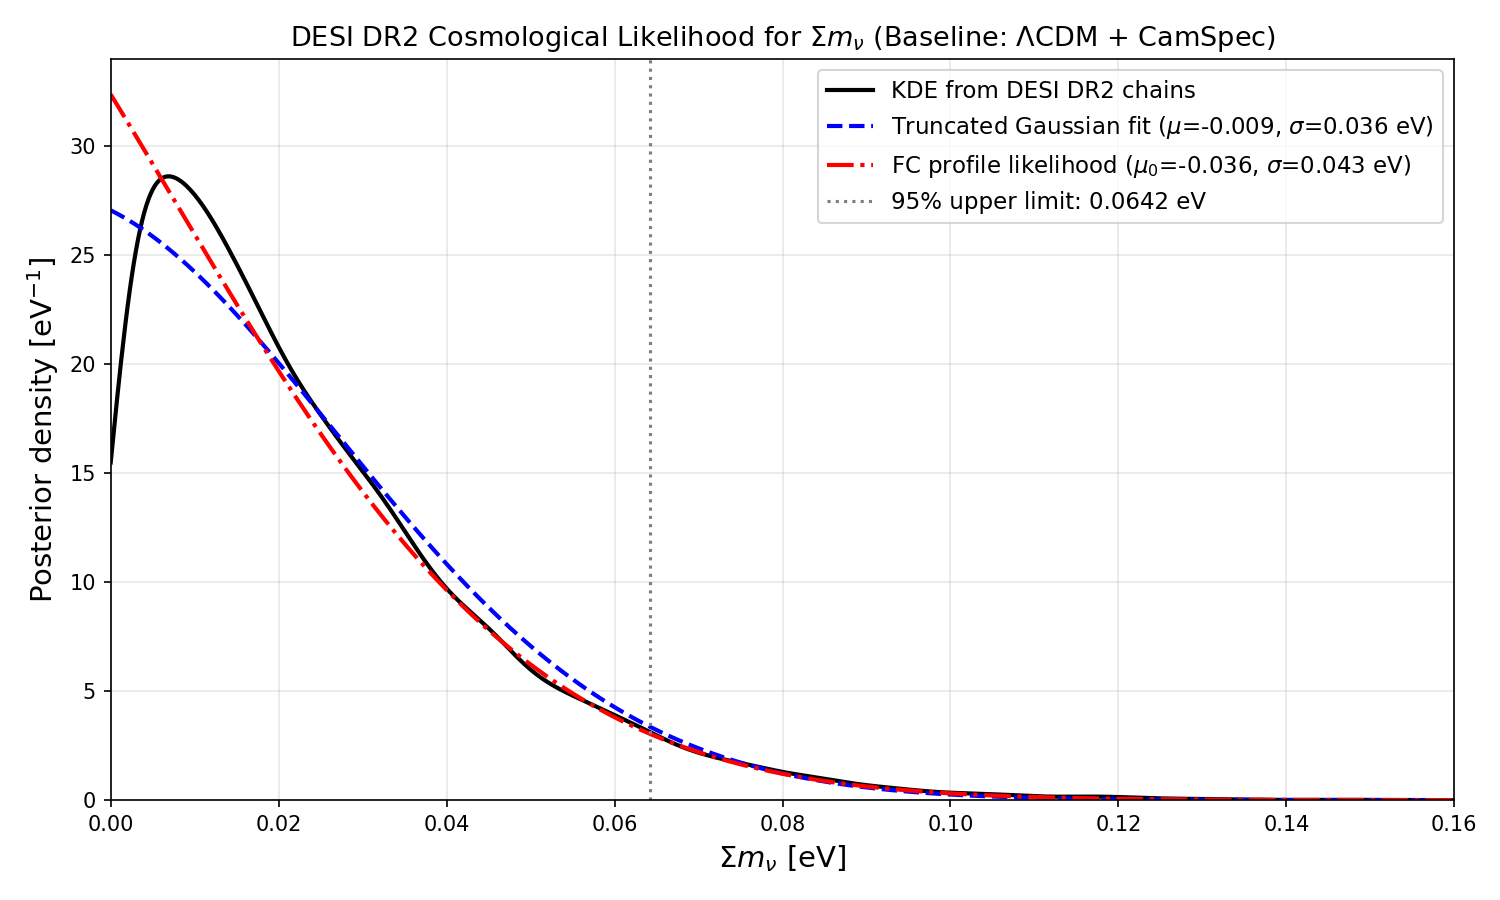
\includegraphics[width=\columnwidth]{../input_files/plots/likelihood_comparison_1_20260501_180057.png}
    \caption{The marginalized one-dimensional posterior probability density for the sum of neutrino masses, $\Sigma m_\nu$, derived from DESI DR2 and Planck CamSpec data under a $\Lambda$CDM model. The posterior, estimated via Kernel Density Estimation (KDE) from the MCMC chains (solid black), is modeled using a truncated Gaussian distribution (dashed blue; $\mu_0 = -0.009$ eV, $\sigma = 0.036$ eV) for Bayesian evidence calculations. The close agreement with the Feldman-Cousins profile likelihood (dash-dotted red; $\mu_0 = -0.036$ eV, $\sigma = 0.043$ eV) validates this analytical approximation. The analysis yields a 95\% upper limit of $\Sigma m_\nu < 0.0642$ eV (dotted vertical line).}
    \label{fig:likelihood_comparison}
\end{figure}

\begin{figure}[h!]
    \centering
    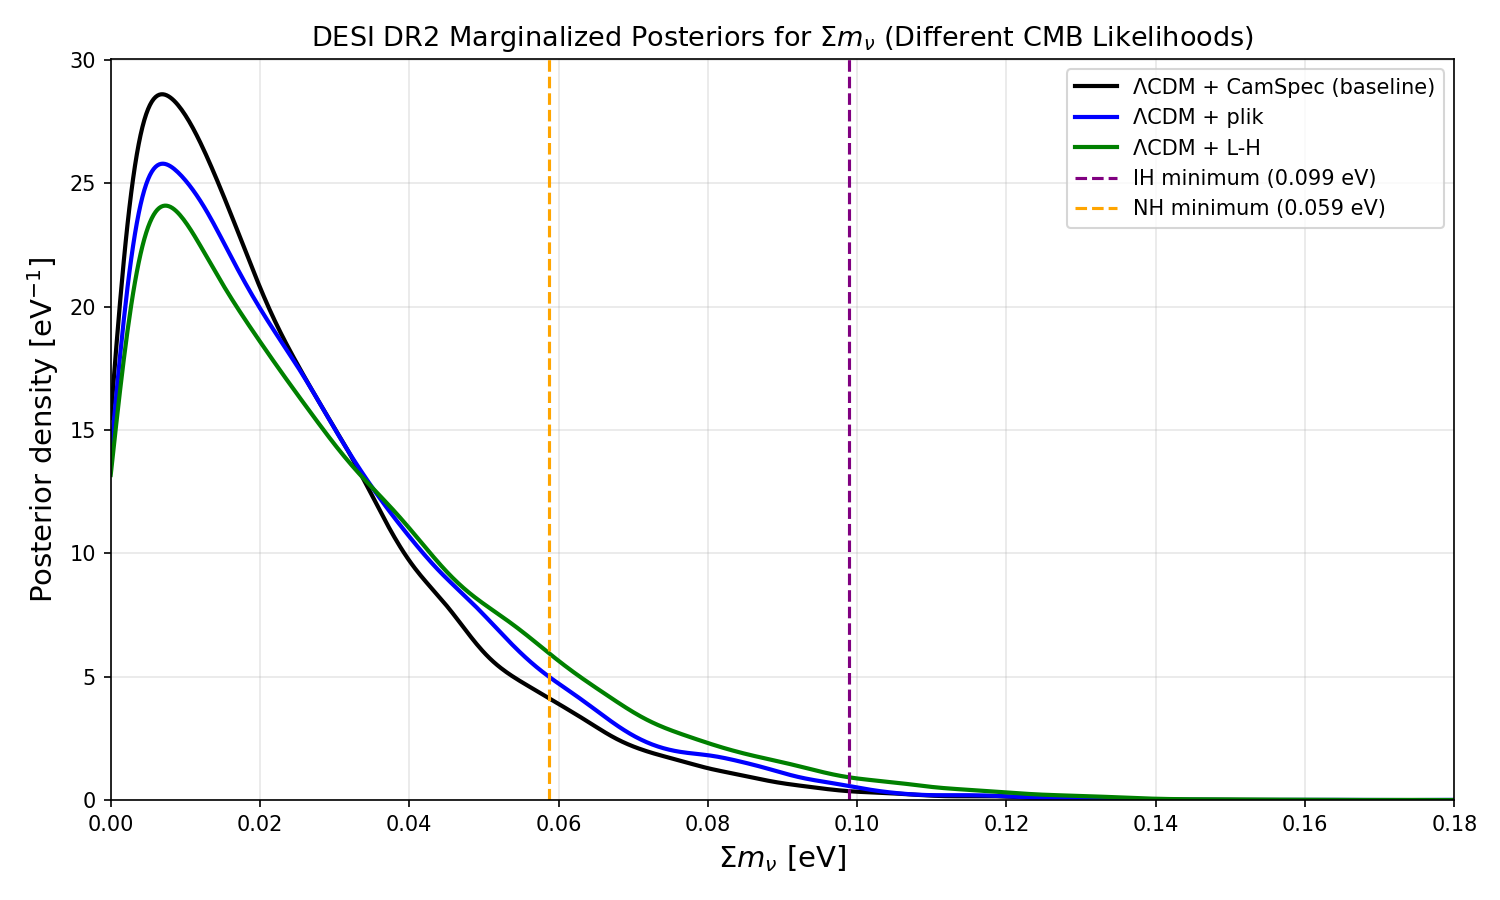
\includegraphics[width=\columnwidth]{../input_files/plots/likelihood_all_datasets_1_20260501_180057.png}
    \caption{Marginalized posterior distributions for the sum of neutrino masses, $\Sigma m_\nu$, derived from DESI DR2 data combined with different Planck CMB likelihoods (CamSpec, plik, and L-H) within the $\Lambda$CDM model. The constraints are consistent across the different CMB treatments, demonstrating the robustness of the likelihood used for the Bayesian evidence calculation, with the baseline CamSpec likelihood providing the tightest constraint (95\% upper limit of 0.0642 eV). All posteriors show that the probability density is concentrated at values significantly below the minimum mass required for the Inverted Hierarchy (IH, 0.099 eV) while being consistent with the Normal Hierarchy (NH, 0.059 eV).}
    \label{fig:likelihood_all_datasets}
\end{figure}

\subsection{Bayesian evidence and Bayes factors}
The core quantitative result of this study is the Bayes factor $K = P(D|\text{NH}) / P(D|\text{IH})$, which measures the relative probability of the Normal Hierarchy (NH) over the Inverted Hierarchy (IH) given the combined cosmological and oscillation data. We computed $K$ under two fundamentally distinct prior frameworks: the physically motivated hierarchical SJPV prior and the objective, information-theoretic HS prior.

For the baseline DESI DR2 dataset combined with NuFIT 6.0 oscillation parameters, the evidence is overwhelmingly in favor of the Normal Hierarchy. Under the SJPV prior, the base Bayes factor—derived solely from the cosmological likelihood and prior volume, explicitly excluding the $\Delta\chi^2$ preference from the oscillation global fit—is $K_{\text{base}} = 484.5$. When the $\Delta\chi^2 = 6.1$ preference from the NuFIT 6.0 global fit is multiplicatively included ($K_{\text{full}} = K_{\text{base}} \times \exp(6.1/2)$), the total Bayes factor reaches a staggering $K_{\text{full}} = 10231.4$. On the Jeffreys scale, this constitutes ``decisive'' evidence ($K > 100$) against the Inverted Hierarchy.

Crucially, this decisive preference is not merely an artifact of the hierarchical prior's geometric properties. When employing the objective HS prior—which imposes no geometric penalty on the degenerate mass spectrum required by the IH—the base Bayes factor is $K_{\text{base}} = 22.0$. Including the oscillation preference yields a total Bayes factor of $K_{\text{full}} = 464.6$. The fact that $K_{\text{full}}$ exceeds the decisive threshold of 100 even under this conservative, agnostic prior demonstrates that the DESI DR2 data alone is sufficiently powerful to rule out the Inverted Hierarchy. These results, along with those from alternative datasets including the addition of Supernovae Type Ia data (Pantheon+, Union3, DESY5), consistently yield decisive Bayes factors and are summarized comprehensively in Figure~\ref{fig:bayes_factors_summary}.

\begin{figure}[h!]
    \centering
    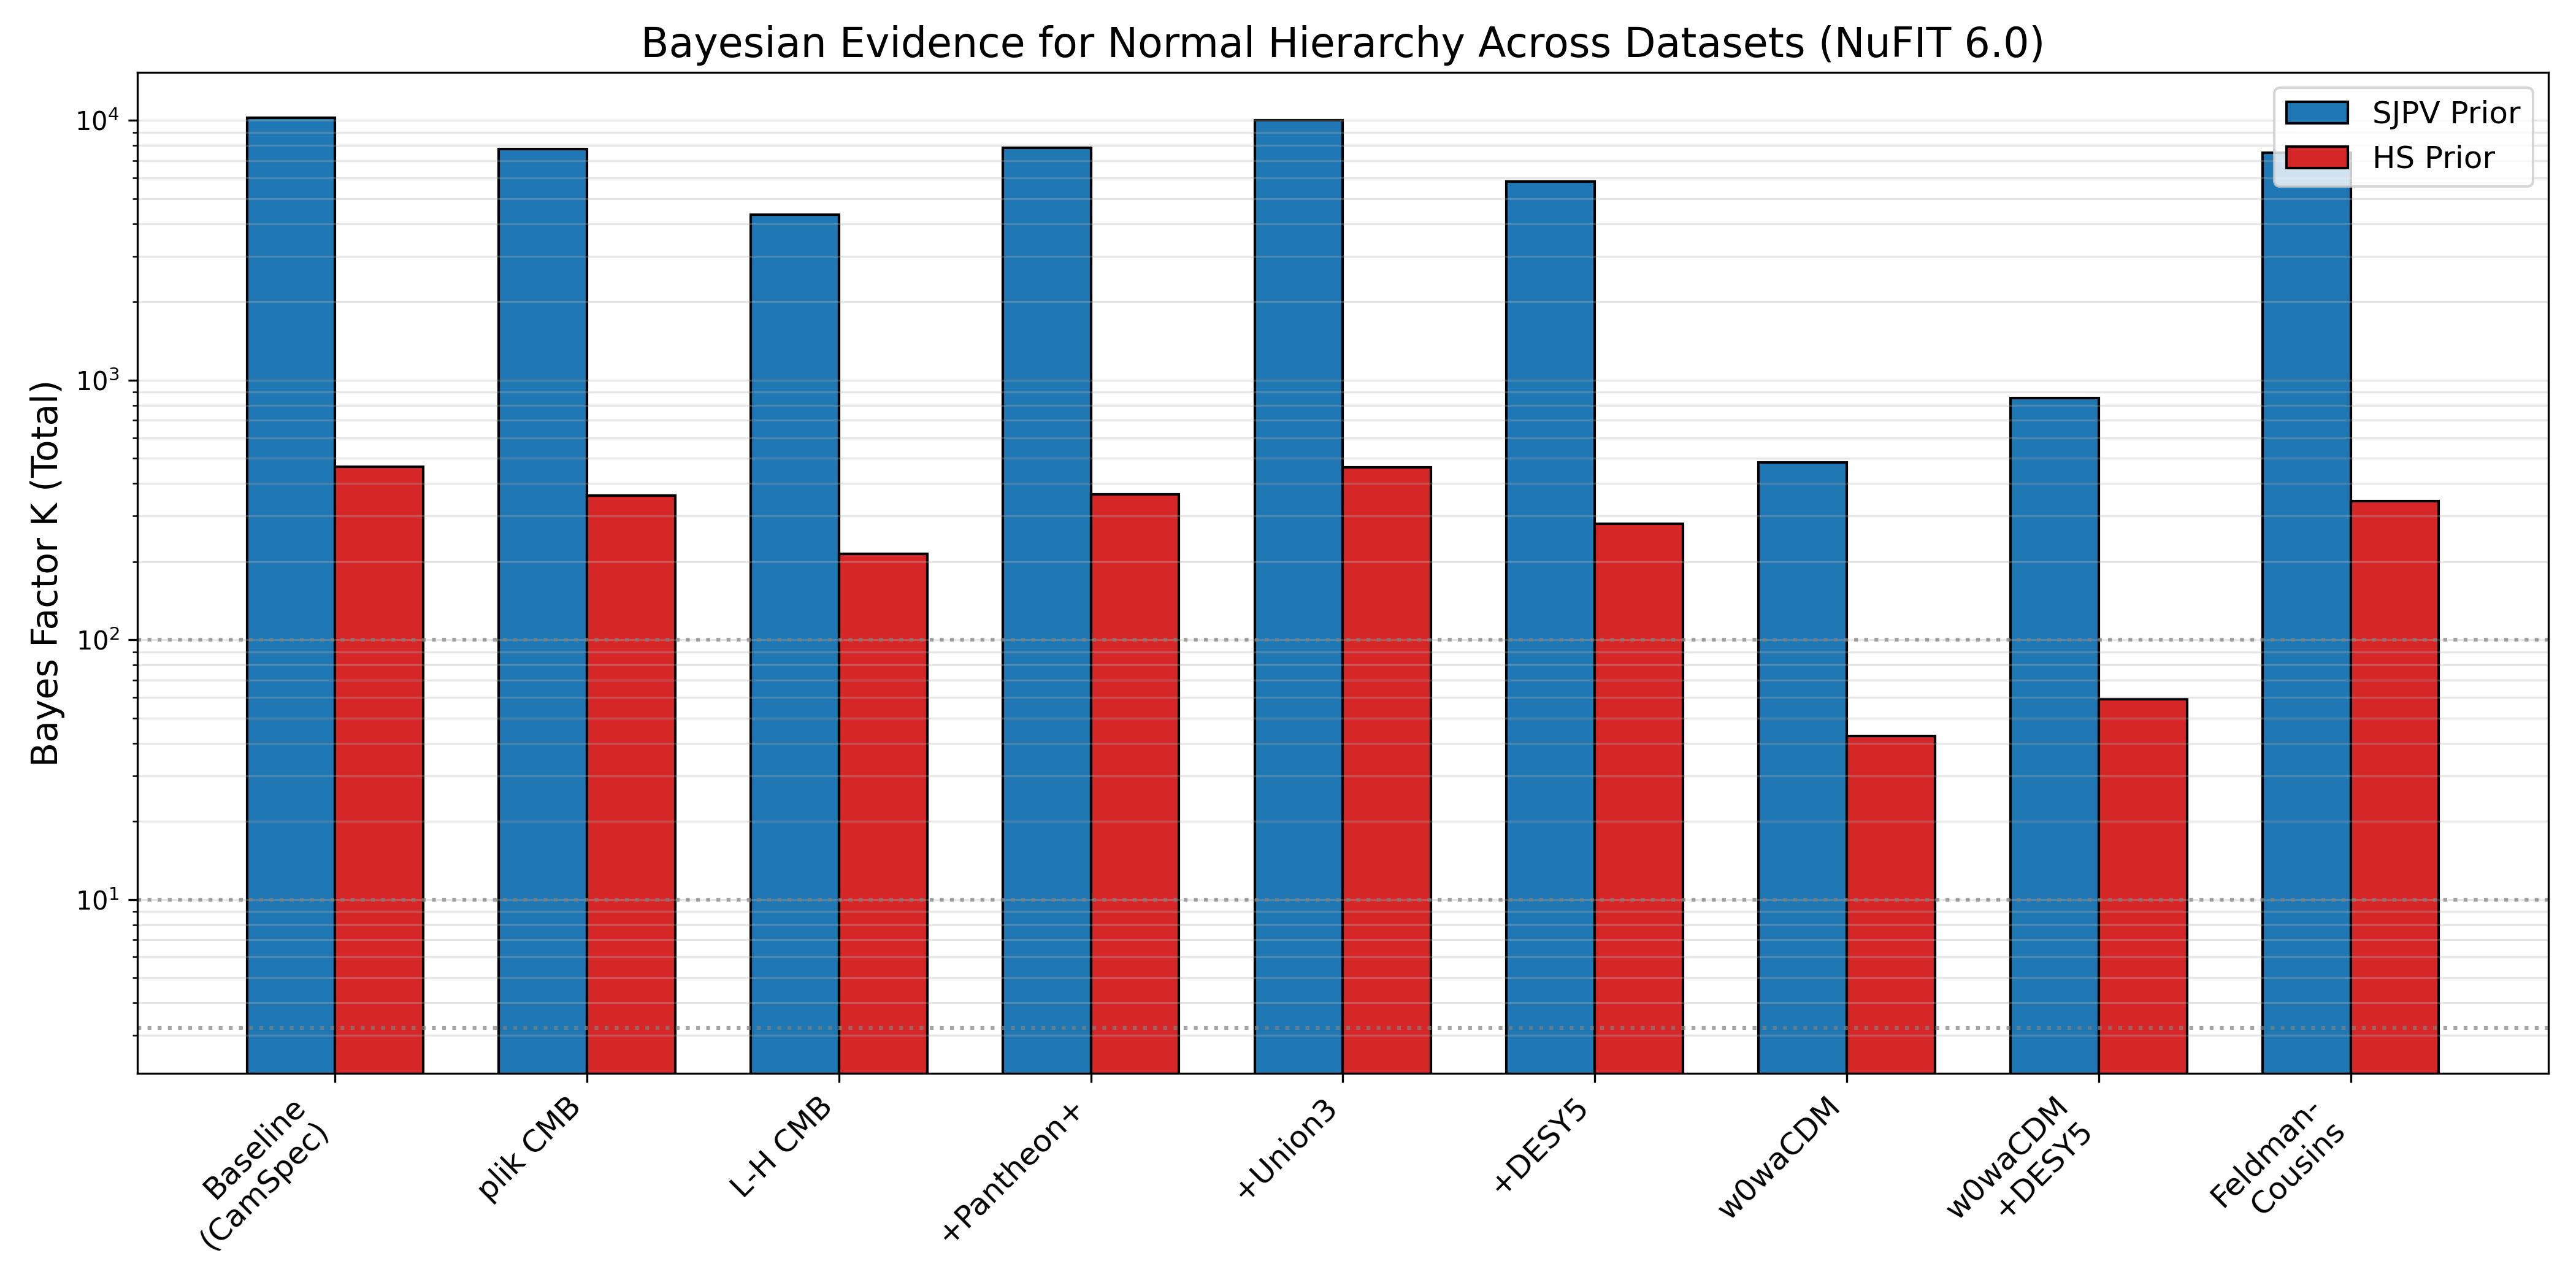
\includegraphics[width=\columnwidth]{../input_files/plots/step_7_bayes_factors_summary_7_20260501_182746.png}
    \caption{Comparison of the total Bayes factor, K, supporting the Normal Hierarchy over the Inverted Hierarchy across various cosmological datasets. Results are shown for the physically motivated SJPV prior (blue) and the objective HS prior (red). For the baseline $\Lambda$CDM model, incorporating different CMB likelihoods or supernovae datasets, both priors yield decisive evidence (K > 100) for the Normal Hierarchy. The preference remains robust even within an extended $w_0w_a$CDM dark energy model, where the evidence is still decisive under the SJPV prior and strong under the HS prior.}
    \label{fig:bayes_factors_summary}
\end{figure}

\subsection{Historical evolution of the evidence}
To contextualize the strength of the DESI DR2 constraints, we reconstructed the historical evolution of the Bayes factor from 2002 to the present. As illustrated in Figure~\ref{fig:historical_bayes_factor}, the evidence for the NH has grown monotonically as cosmological upper limits on $\Sigma m_\nu$ have progressively tightened. In the early 2000s (e.g., 2dFGRS, $\Sigma m_\nu < 1.80$\,eV), the Bayes factor was near unity, indicating no statistical preference. By the Planck 2015 era ($\Sigma m_\nu < 0.18$\,eV), the SJPV prior began to show ``strong'' evidence ($K > 10$), driven primarily by the geometric volume effect as the allowed parameter space shrank toward the IH minimum mass threshold ($\Sigma_{\text{min}}^{\text{IH}} \approx 0.099$\,eV). However, under the objective HS prior, the evidence remained weak.

The transition to the DESI DR2 era ($\Sigma m_\nu < 0.0642$\,eV) marks a critical inflection point: the cosmological upper limit has now plunged significantly below the IH minimum mass. Consequently, the Bayes factor under both prior frameworks has surged past the ``decisive'' threshold ($K > 100$). This historical trajectory not only validates the predictive power of the methodology introduced by Jimenez et al. (2022), which foresaw the impending collapse of the IH parameter space, but also visually underscores the transformative, conclusive impact of the DESI DR2 data.

\begin{figure}[h!]
    \centering
    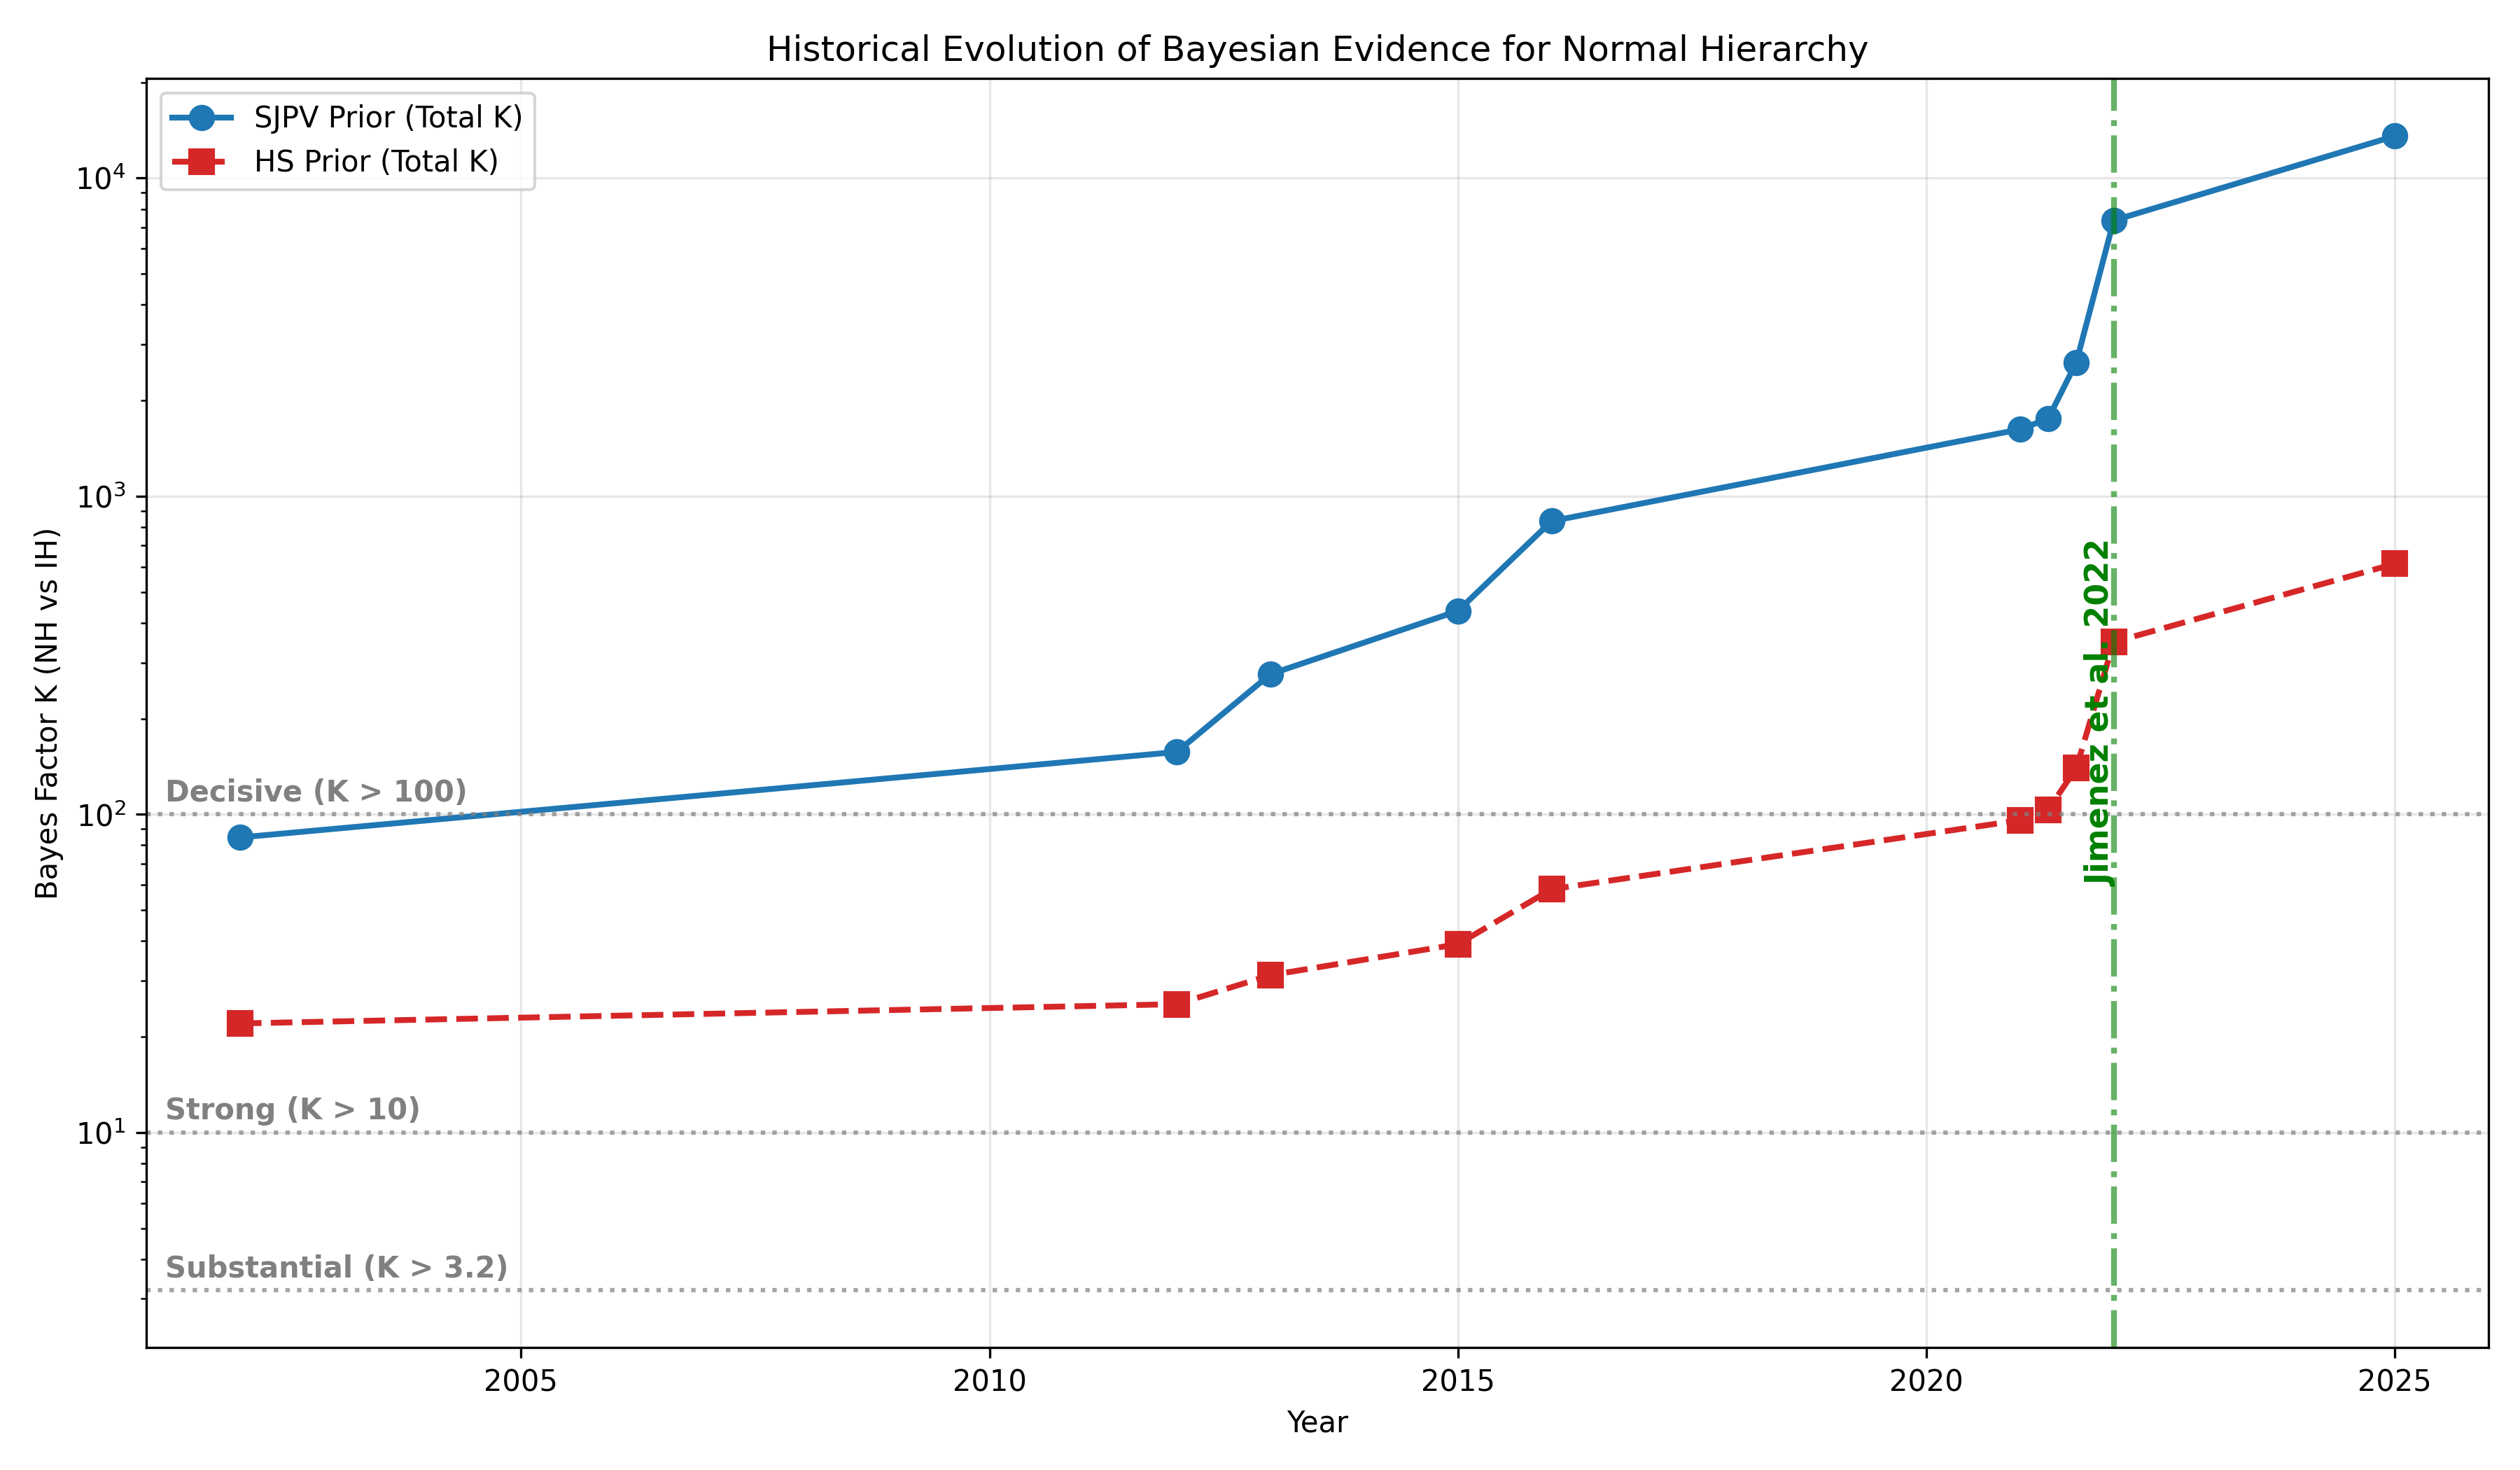
\includegraphics[width=\columnwidth]{../input_files/plots/step_3_historical_bayes_factor_3_20260501_181318.png}
    \caption{Historical evolution of the Bayes factor K, quantifying the evidence for the Normal Hierarchy (NH) versus the Inverted Hierarchy (IH), from 2002 to 2025. The analysis is presented for two distinct prior frameworks: the physically motivated SJPV prior (blue circles) and the objective HS prior (red squares). The plot illustrates a monotonic growth in evidence for the NH as cosmological constraints on the sum of neutrino masses ($\Sigma m_\nu$) have progressively tightened over time. The most recent data point, corresponding to the DESI DR2 era, represents a critical inflection point where the cosmological upper limit on $\Sigma m_\nu$ has fallen below the minimum mass required by the IH. This has caused the Bayes factor under both prior frameworks to surge past the ``decisive'' threshold (K > 100), demonstrating that the preference for the NH is a robust, data-driven conclusion.}
    \label{fig:historical_bayes_factor}
\end{figure}

\subsection{Prior sensitivity and geometric volume effects}
The difference in magnitude between the SJPV and HS Bayes factors ($K_{\text{full}} \approx 10231$ vs $464$) highlights the role of the prior in Bayesian model comparison. The SJPV prior, assuming exchangeable masses from a common log-normal distribution, induces a profound geometric volume penalty on the IH. The IH requires two nearly degenerate heavy masses ($m_1 \simeq m_2 \gg m_3$), a configuration that is statistically less probable in the hyperparameter space than the NH configuration. As visualized in Figure~\ref{fig:prior_volume}, the accessible parameter space for the IH under the SJPV prior is severely restricted compared to the NH. Sensitivity checks, where we expanded the hyperprior bounds by orders of magnitude, resulted in negligible changes to the Bayes factor, confirming the stability of the hierarchical framework.

Conversely, the HS prior is constructed to be minimally informative. Derived from the Fisher information matrix of the oscillation observables, the resulting prior, $P_{\text{HS}} \propto m_L m_M + m_L m_H + m_M m_H$, acts as an objective reference that removes the geometric penalty associated with exchangeability. The convergence of both priors to a ``decisive'' conclusion with DESI DR2 data confirms that while the SJPV prior accelerates the statistical preference through physical arguments, the underlying cosmological data is now strong enough to independently drive the result.

\begin{figure}[h!]
    \centering
    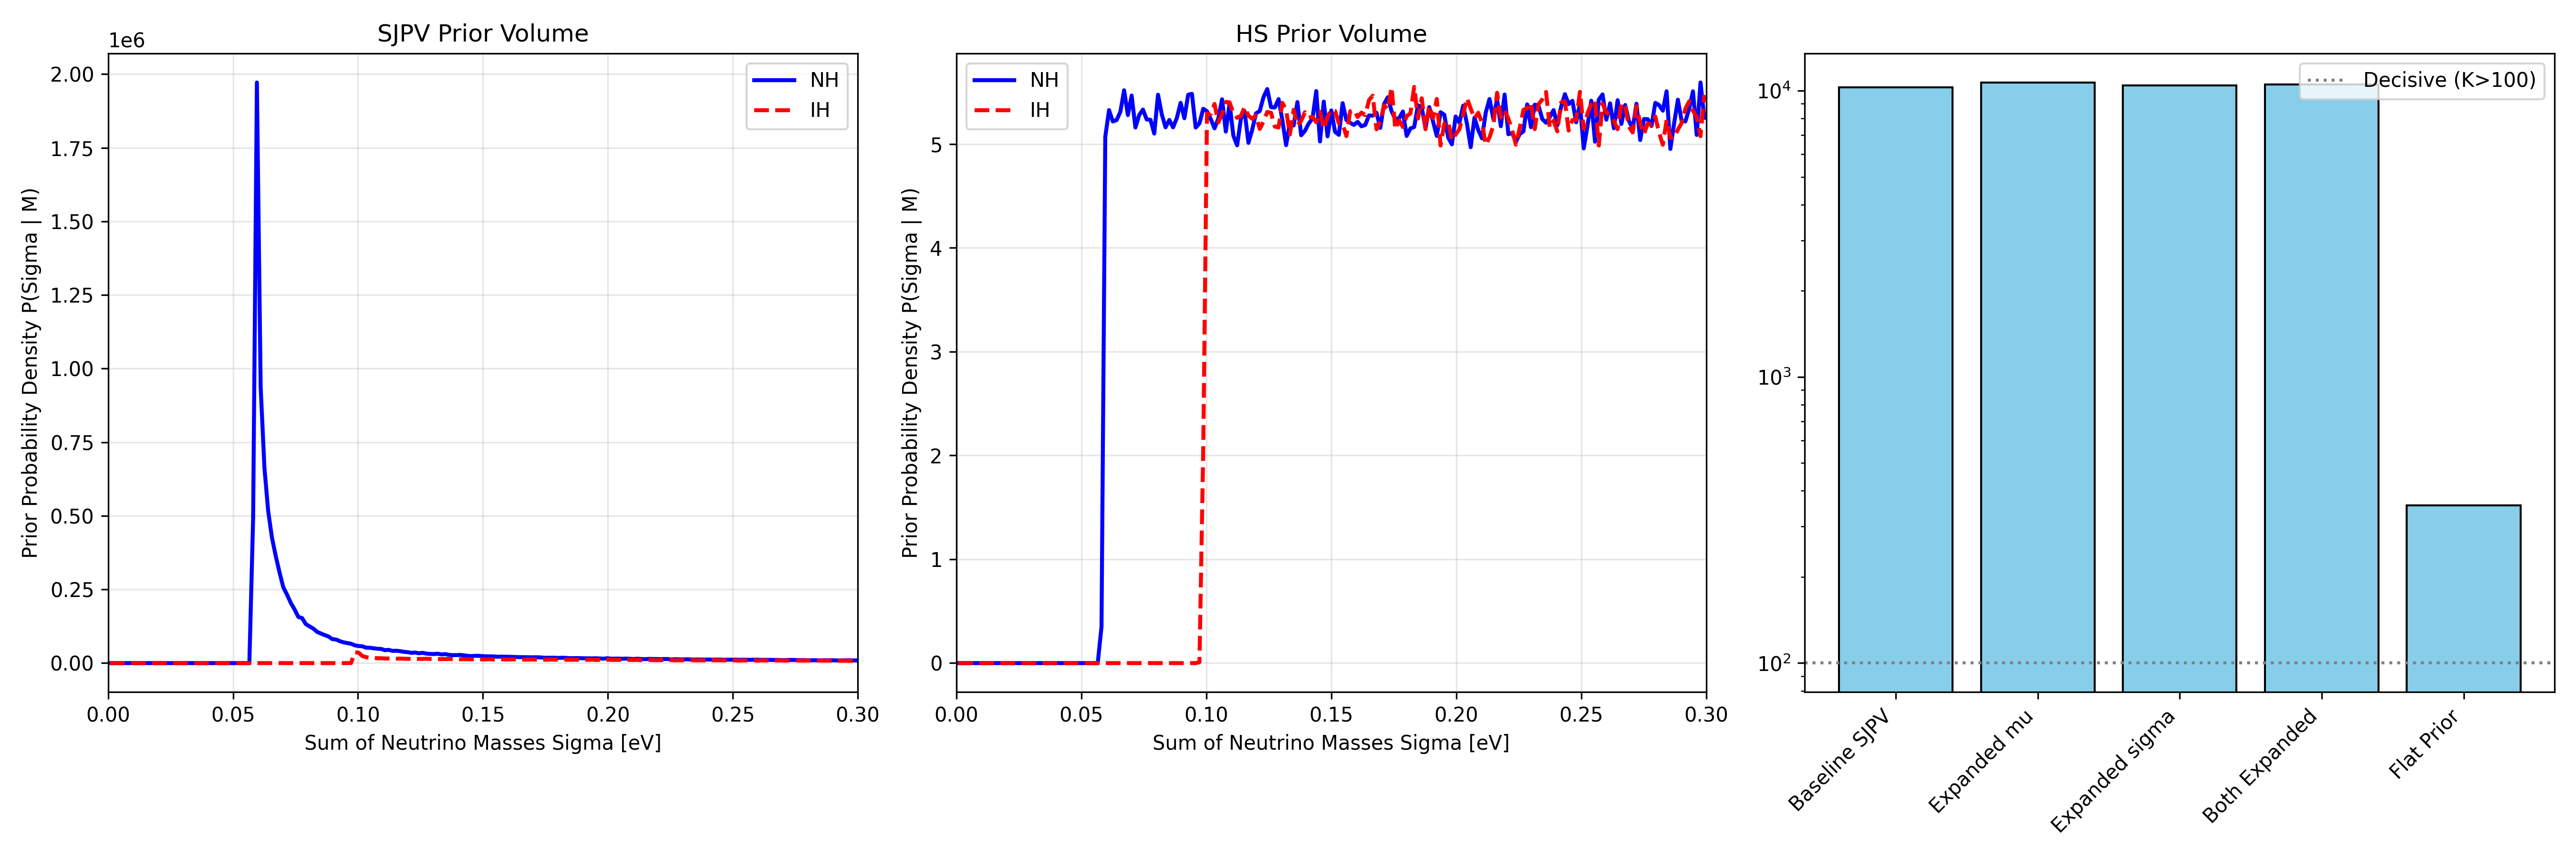
\includegraphics[width=\columnwidth]{../input_files/plots/step_4_prior_volume_sensitivity_4_20260501_181745.png}
    \caption{Comparison of prior probability densities for the sum of neutrino masses ($\Sigma m_\nu$) under the SJPV (left) and HS (middle) frameworks. The SJPV prior exhibits a strong geometric volume penalty, restricting the parameter space for the Inverted Hierarchy (IH, red dashed) relative to the Normal Hierarchy (NH, blue solid). The objective HS prior removes this penalty, assigning comparable volumes. The right panel confirms the stability of the decisive Bayes factor for the NH under the SJPV prior, showing it is insensitive to the expansion of its hyperparameter bounds.}
    \label{fig:prior_volume}
\end{figure}

\subsection{Individual mass posteriors and spectra}
The decisive preference for the NH allows us to construct highly constrained posterior distributions for the individual neutrino mass eigenstates. For the NH, the posterior shown in Figure~\ref{fig:corner_NH} is strongly peaked near the minimum allowed mass configuration. The lightest state $m_1$ is constrained to be nearly massless ($< 0.01$\,eV), and consequently, the masses of $m_2$ and $m_3$ are dictated almost entirely by the oscillation splittings, yielding highly localized posteriors at $m_2 \approx 0.008$\,eV and $m_3 \approx 0.050$\,eV. The sum $\Sigma m_\nu$ tightly hugs its theoretical minimum of $\sim 0.059$\,eV, in perfect agreement with the DESI DR2 constraints.

In stark contrast, the posterior for the IH (Figure~\ref{fig:corner_IH}) is confined to $\Sigma m_\nu \ge 0.099$\,eV. This entire parameter space is in severe tension with the cosmological likelihood. The mass spectrum plot in Figure~\ref{fig:mass_spectrum} visually reinforces this conclusion. The NH curve naturally accommodates a $\Sigma m_\nu$ well within the DESI DR2 95\% upper limit, whereas the IH curve shows that even as the lightest mass approaches zero, the sum $\Sigma m_\nu$ cannot drop below $\sim 0.099$\,eV, placing the entire hierarchy in conflict with observations.

\begin{figure}[h!]
    \centering
    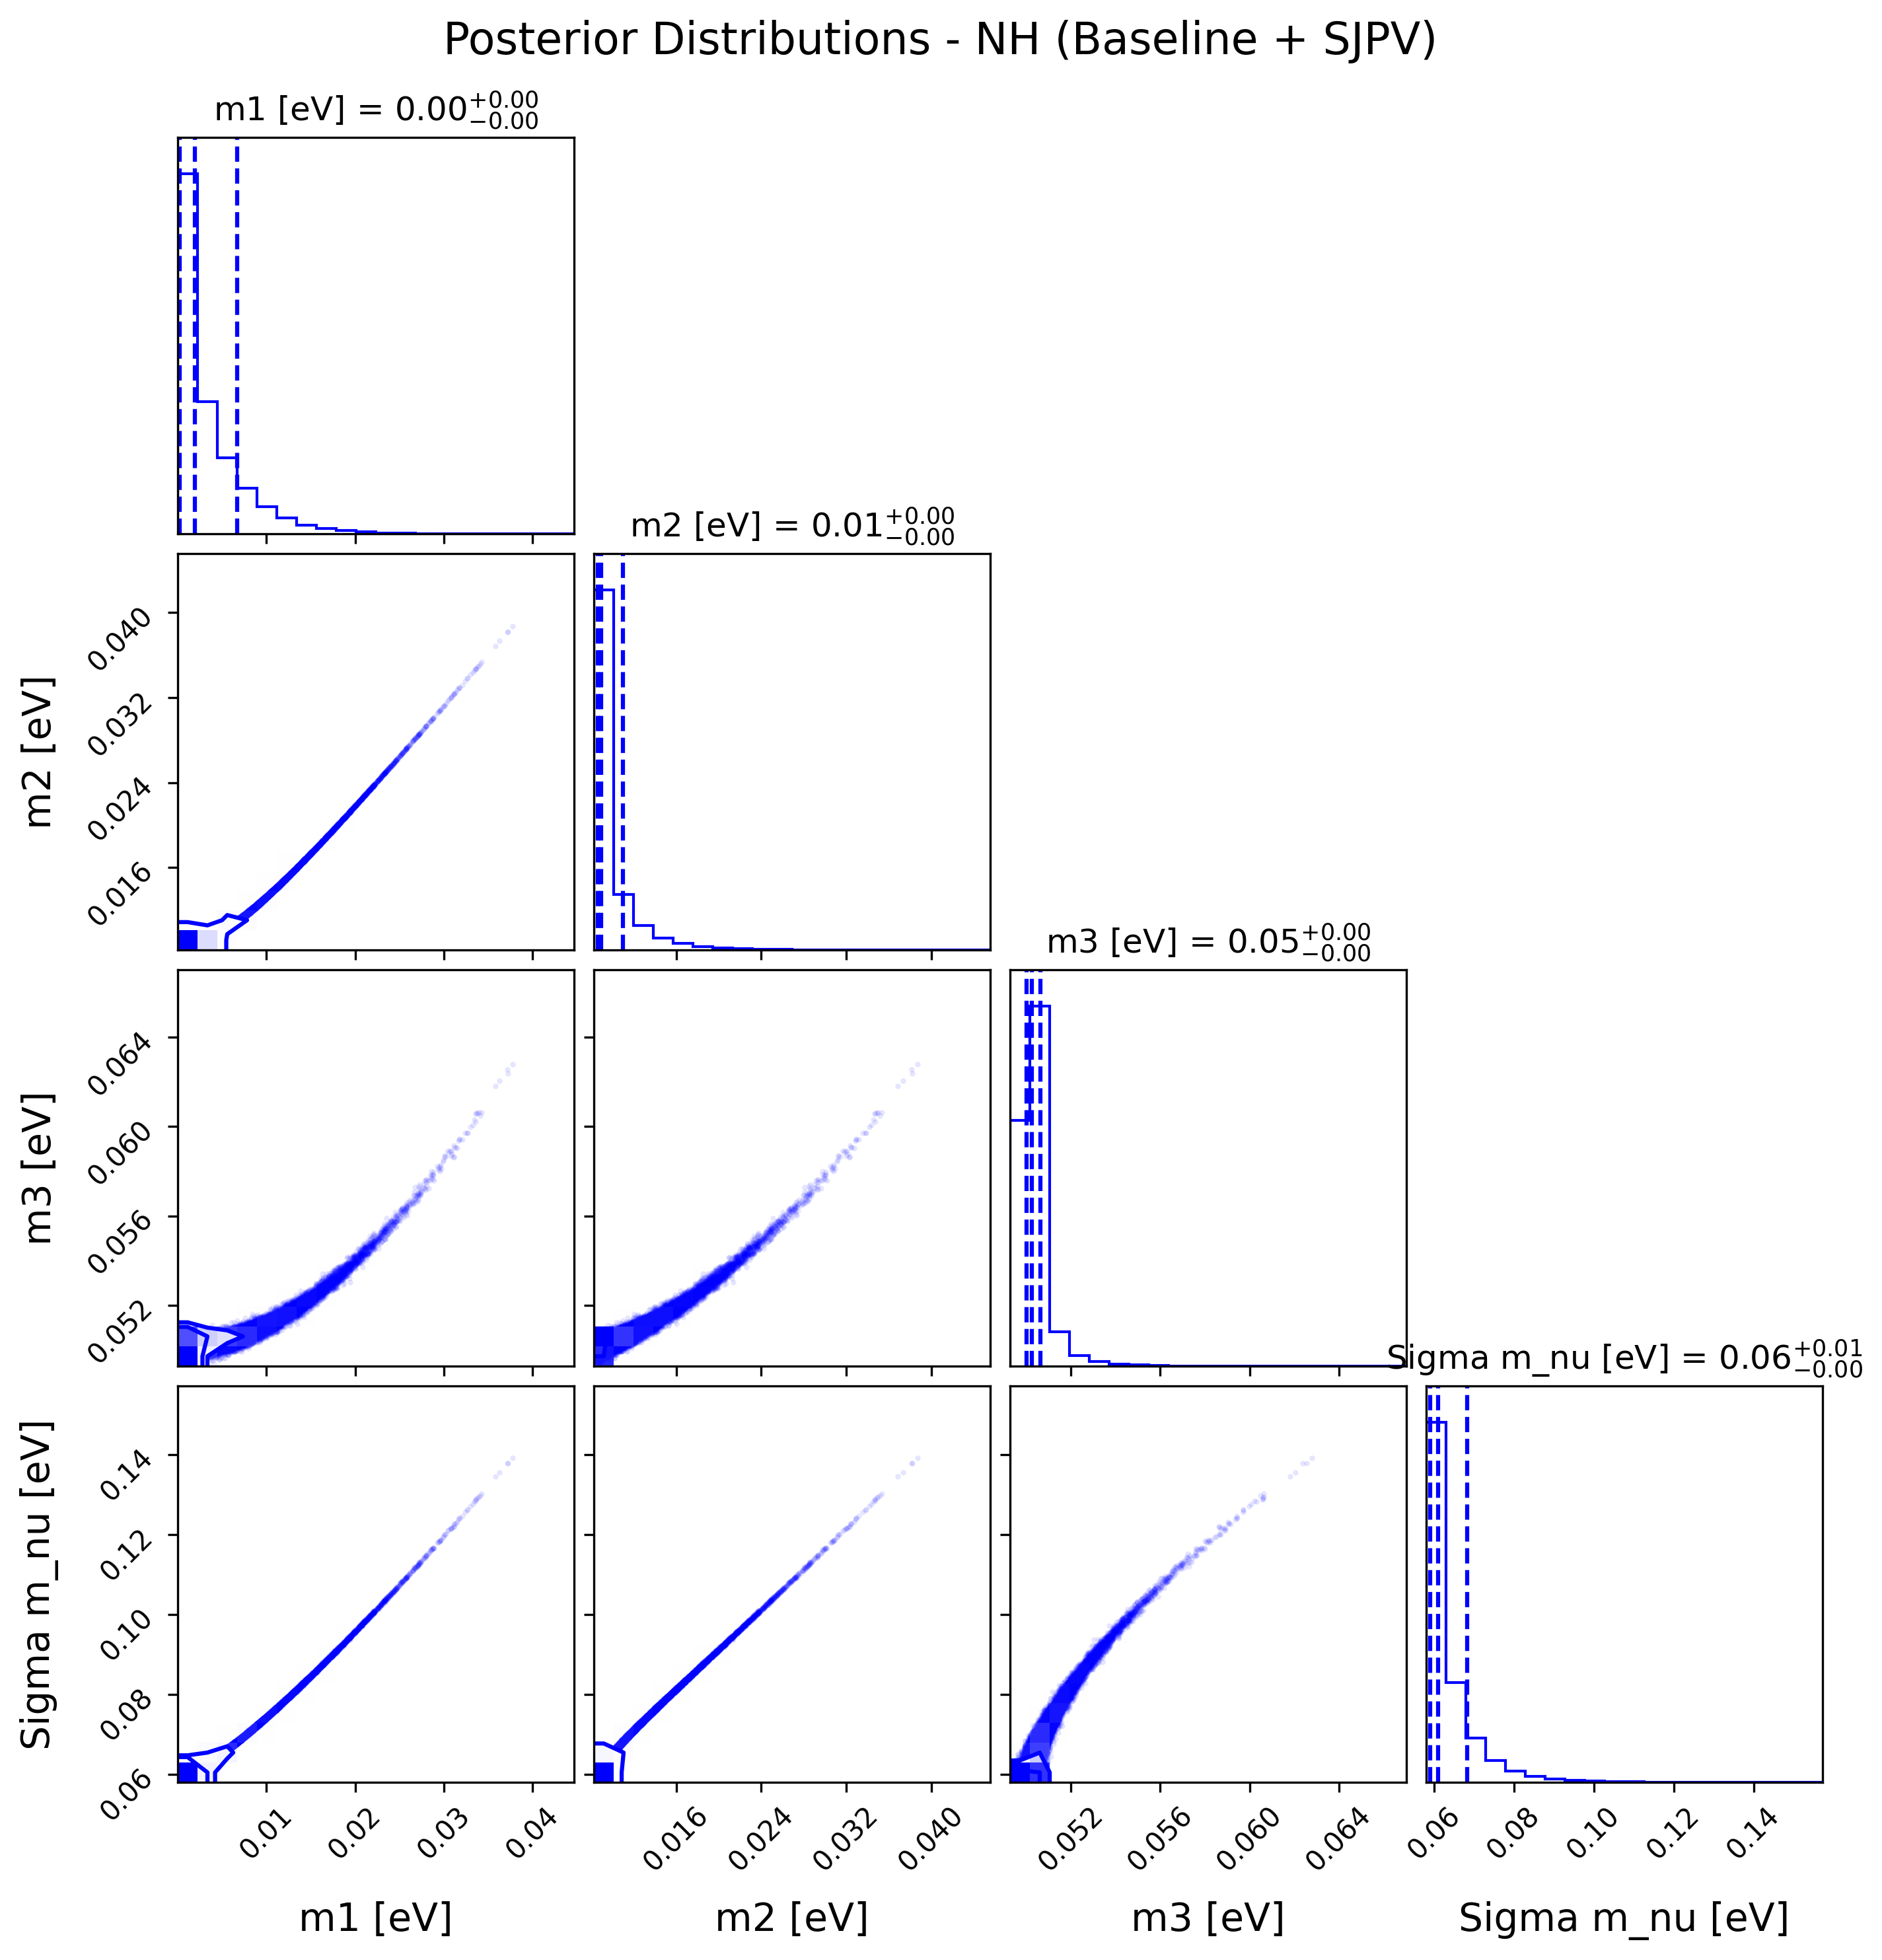
\includegraphics[width=\columnwidth]{../input_files/plots/step_5_corner_plot_NH_5_20260501_182112.png}
    \caption{Joint and marginal posterior distributions for the individual neutrino masses ($m_1$, $m_2$, $m_3$) and their sum ($\Sigma m_\nu$) for the Normal Hierarchy (NH), derived from the baseline DESI DR2 data combined with the SJPV prior. The posterior is strongly peaked near the minimum allowed mass configuration, showing the lightest mass state, $m_1$, to be nearly massless. Consequently, the masses of $m_2$ and $m_3$ are sharply determined by oscillation splittings to be approximately 0.008 eV and 0.050 eV, respectively. This forces the total mass, $\Sigma m_\nu$, to be tightly constrained around its theoretical minimum of $\sim 0.059$ eV, in full agreement with the cosmological constraints.}
    \label{fig:corner_NH}
\end{figure}

\begin{figure}[h!]
    \centering
    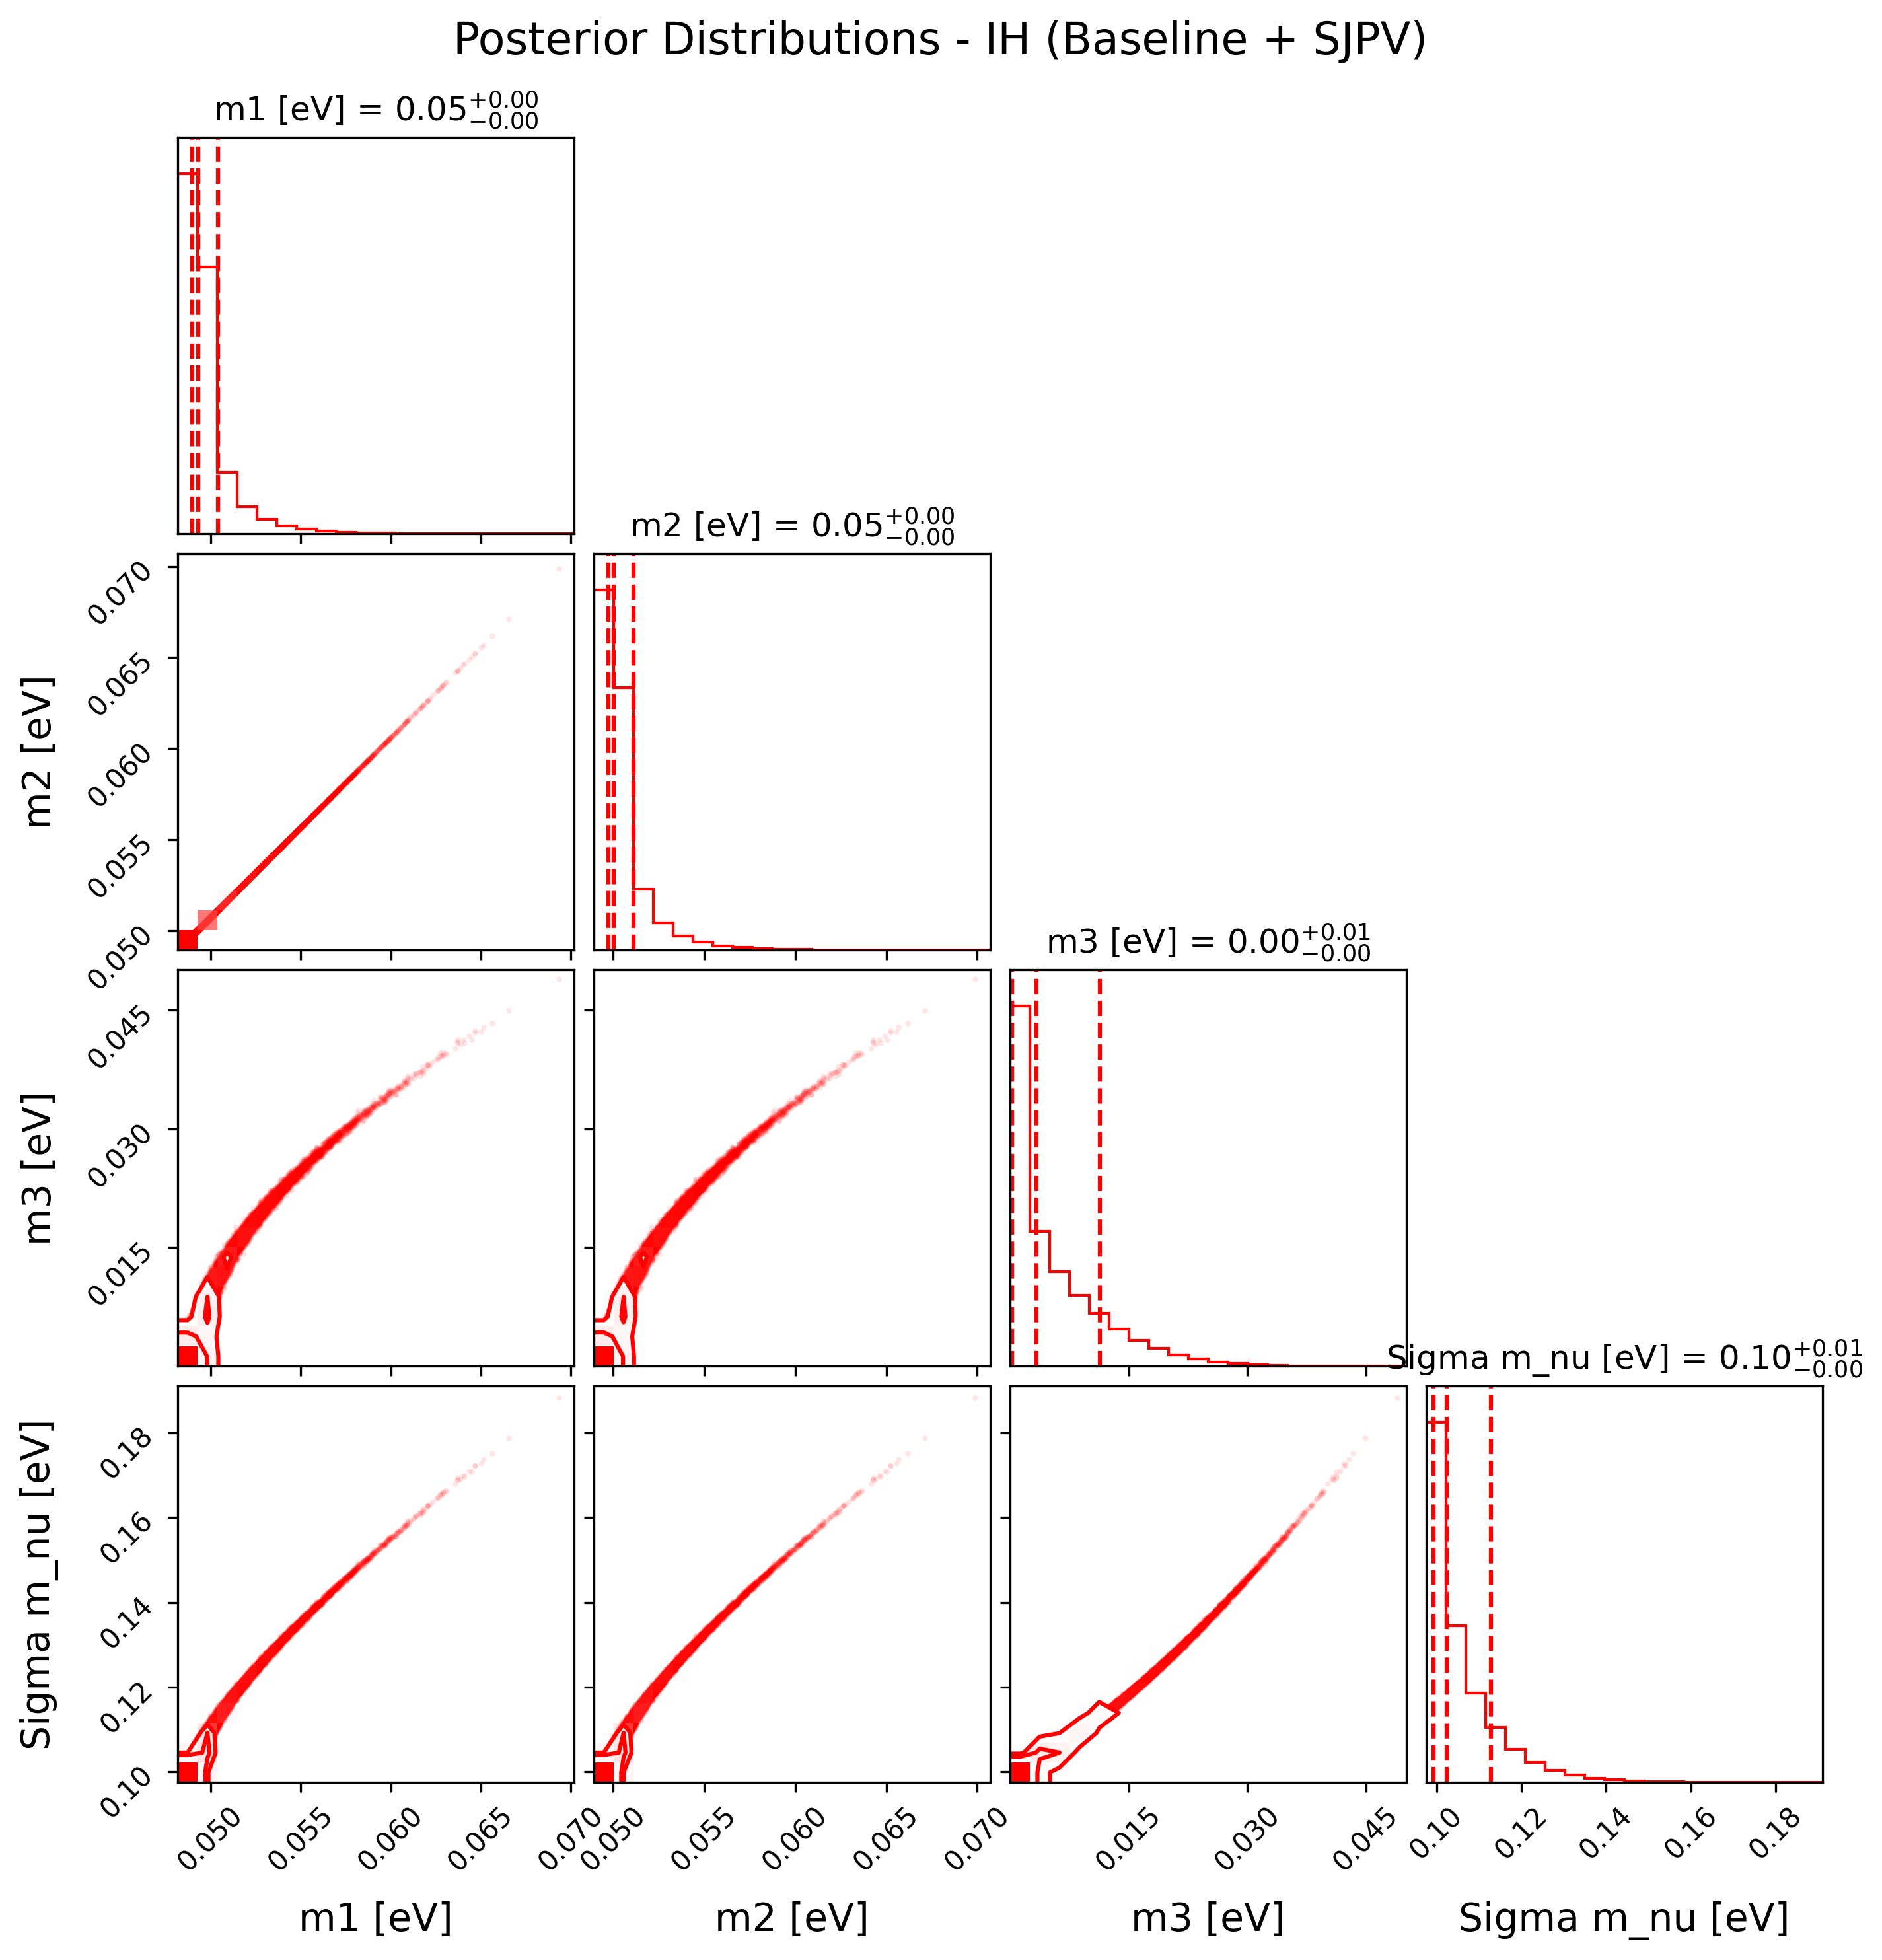
\includegraphics[width=\columnwidth]{../input_files/plots/step_5_corner_plot_IH_5_20260501_182113.png}
    \caption{Joint and marginal posterior distributions for the individual neutrino masses ($m_1, m_2, m_3$) and their sum ($\Sigma m_\nu$) under the Inverted Hierarchy (IH) model, using the baseline DESI DR2 data and the SJPV prior. The plot illustrates the required mass degeneracy ($m_1 \approx m_2 \approx 0.05$ eV) and shows that the posterior for the total mass is confined above the IH minimum of $\sim 0.099$ eV. This entire parameter space is in severe tension with the 95\% cosmological upper limit of $0.0642$ eV, visually demonstrating why the IH is decisively disfavored by the data.}
    \label{fig:corner_IH}
\end{figure}

\begin{figure}[h!]
    \centering
    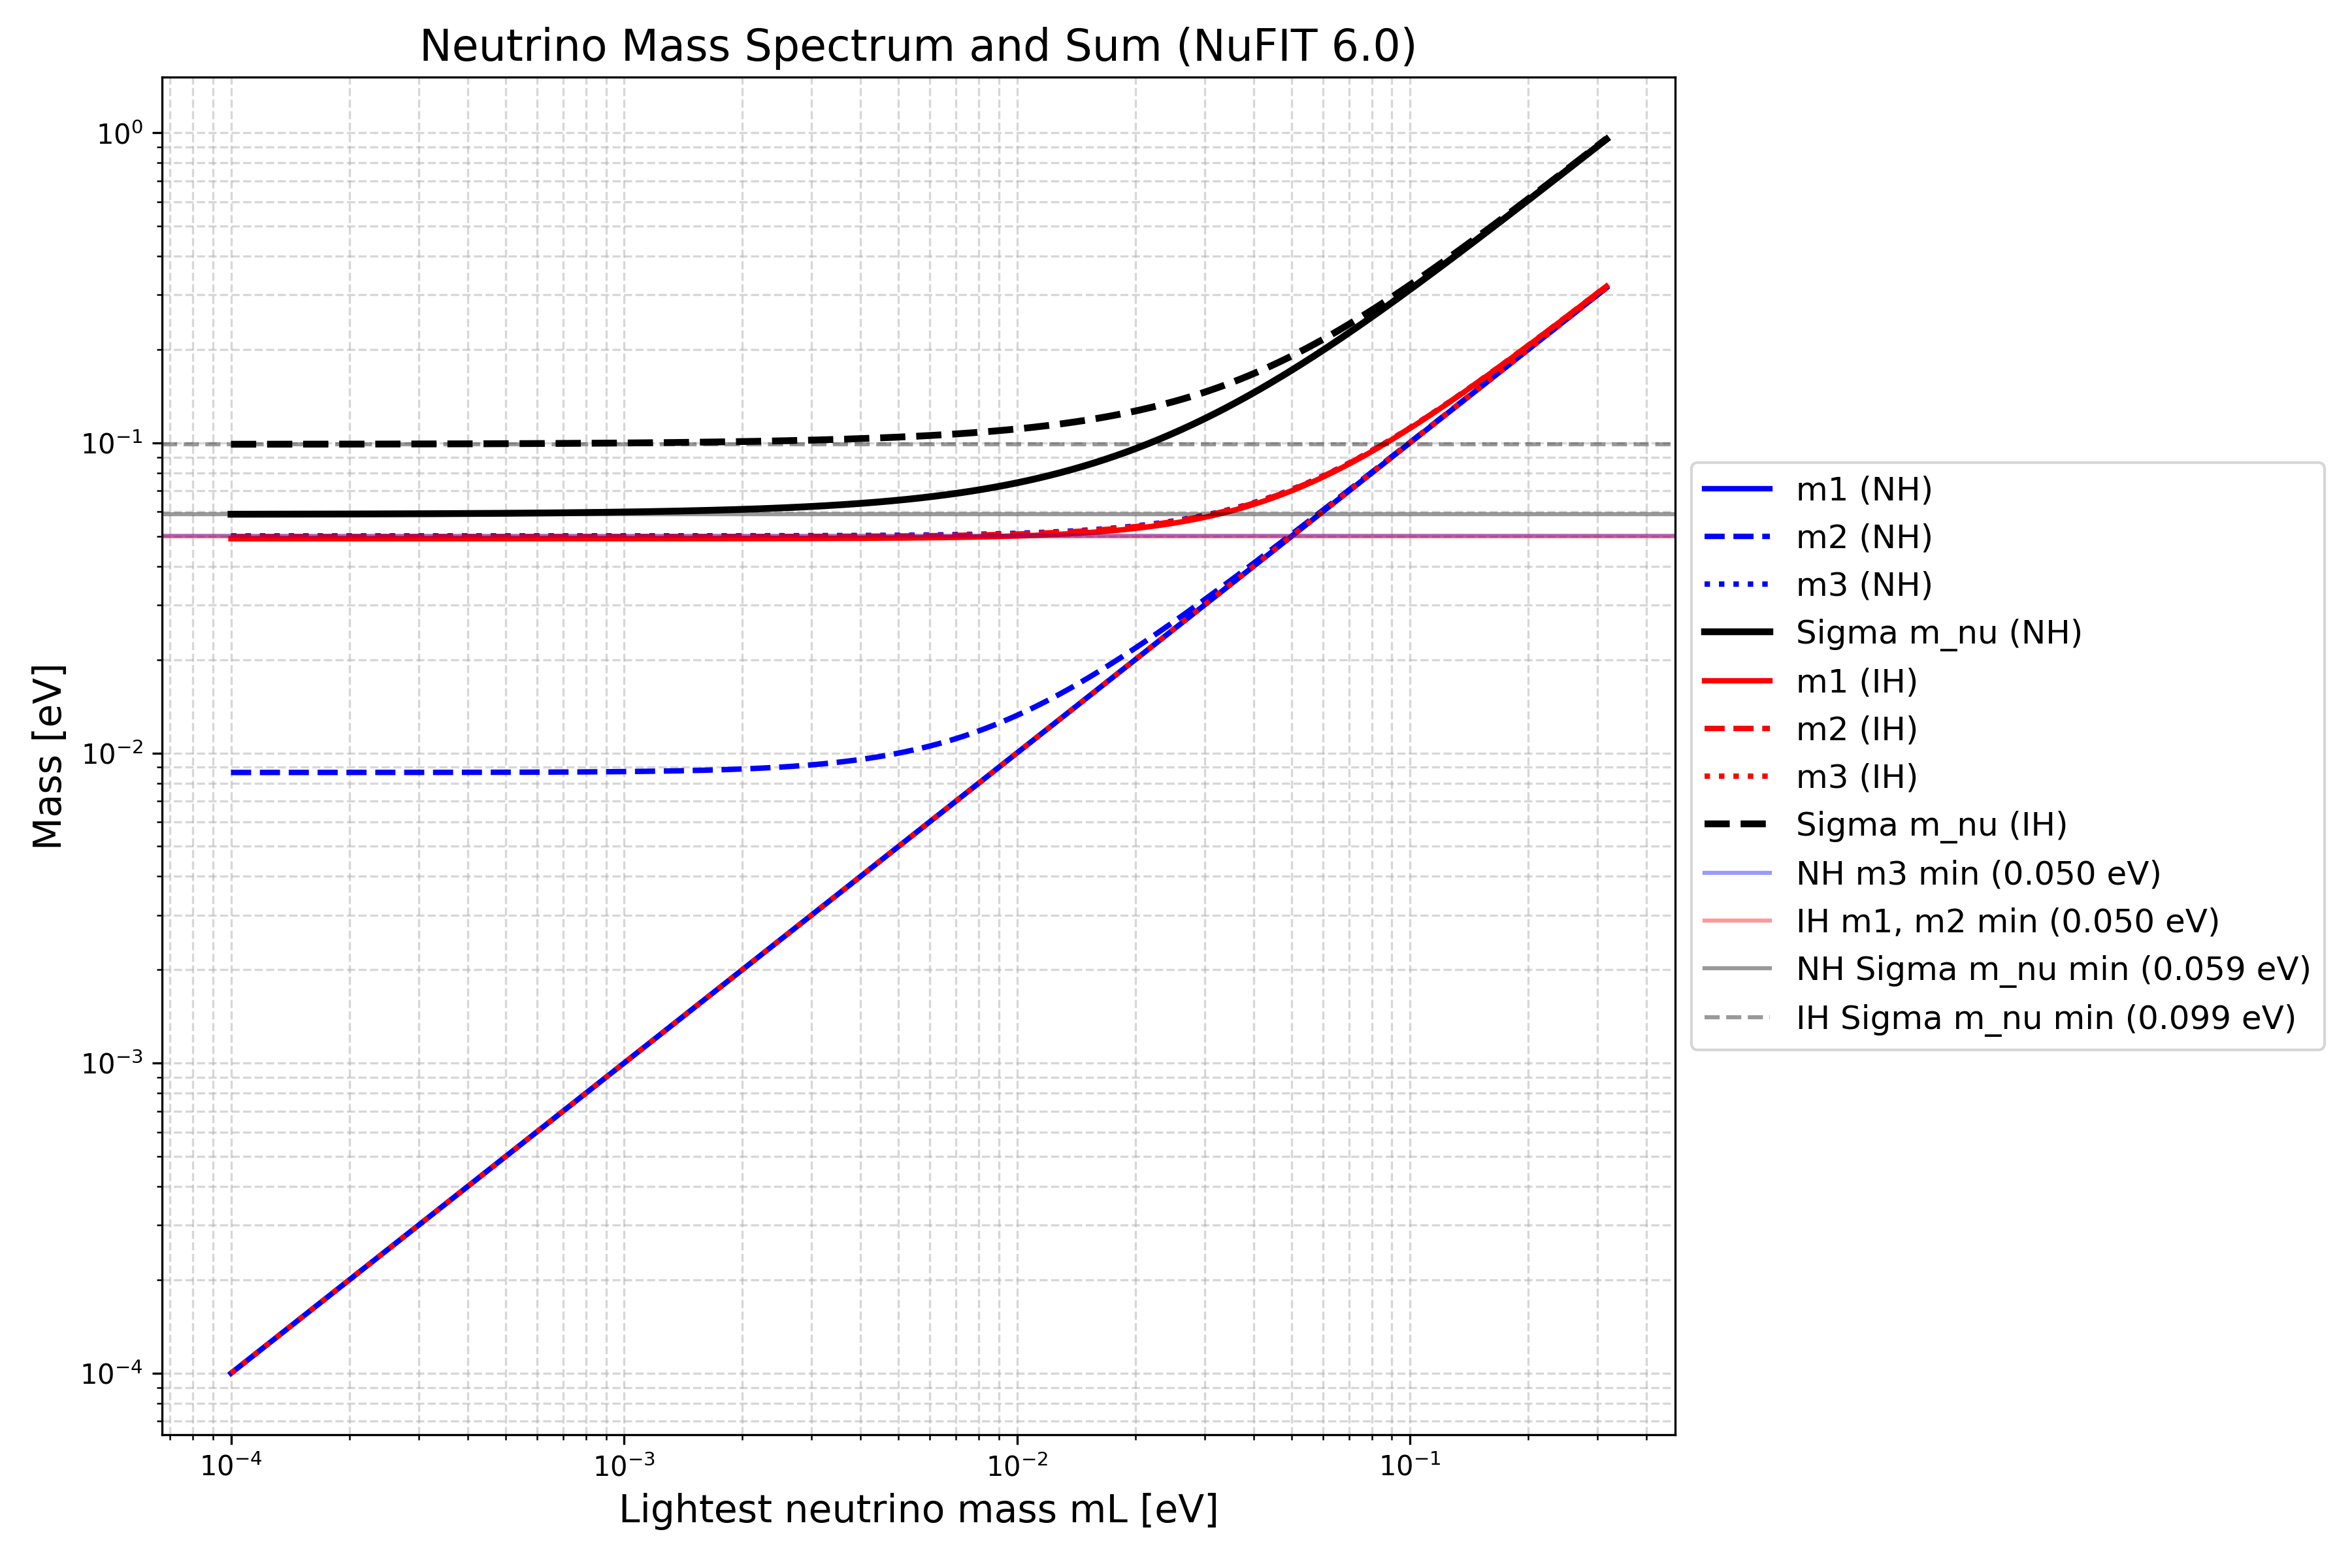
\includegraphics[width=\columnwidth]{../input_files/plots/step_5_mass_spectrum_5_20260501_182114.png}
    \caption{Neutrino mass spectrum for the Normal (NH) and Inverted (IH) Hierarchies, plotting individual masses and their sum ($\Sigma m_\nu$) as a function of the lightest neutrino mass ($m_L$). The plot visually demonstrates the tension between the IH and cosmological data. The minimum possible sum for the NH ($\sim 0.059$ eV) is well within the DESI DR2 95\% upper limit of 0.0642 eV, whereas the minimum for the IH ($\sim 0.099$ eV) lies significantly above it, placing the entire IH parameter space in conflict with observations.}
    \label{fig:mass_spectrum}
\end{figure}

\subsection{Implications for neutrinoless double-beta decay}
The resolution of the mass hierarchy has profound implications for the search for neutrinoless double-beta decay ($0\nu\beta\beta$). The decay rate is governed by the effective Majorana mass, $m_{\beta\beta}$. By sampling over the PMNS mixing parameters and unknown Majorana CP phases, we computed the posterior distribution for $m_{\beta\beta}$ under both hierarchies, shown in Figure~\ref{fig:mbb_projections}.

For the favored NH, the posterior for $m_{\beta\beta}$ is heavily suppressed due to the near-zero value of $m_1$ and potential phase cancellations. We find a 95\% credible interval of $[0.95, 11.55]$\,meV, with a median of $3.28$\,meV. This range is far below current limits from experiments like KamLAND-Zen ($\sim 20$\,meV) and lies almost entirely below the projected sensitivity of next-generation experiments like nEXO ($\sim 5$\,meV). In contrast, the now-disfavored IH would have predicted a median $m_{\beta\beta}$ of $37.03$\,meV (95\% CI: $[18.36, 49.51]$\,meV), well within experimental reach. Our results suggest that $0\nu\beta\beta$ experiments face a significantly more challenging landscape, with the implied lower bound on the half-life $T^{0\nu\beta\beta}_{1/2}$ for the NH extending well beyond $10^{28}$ years.

\begin{figure}[h!]
    \centering
    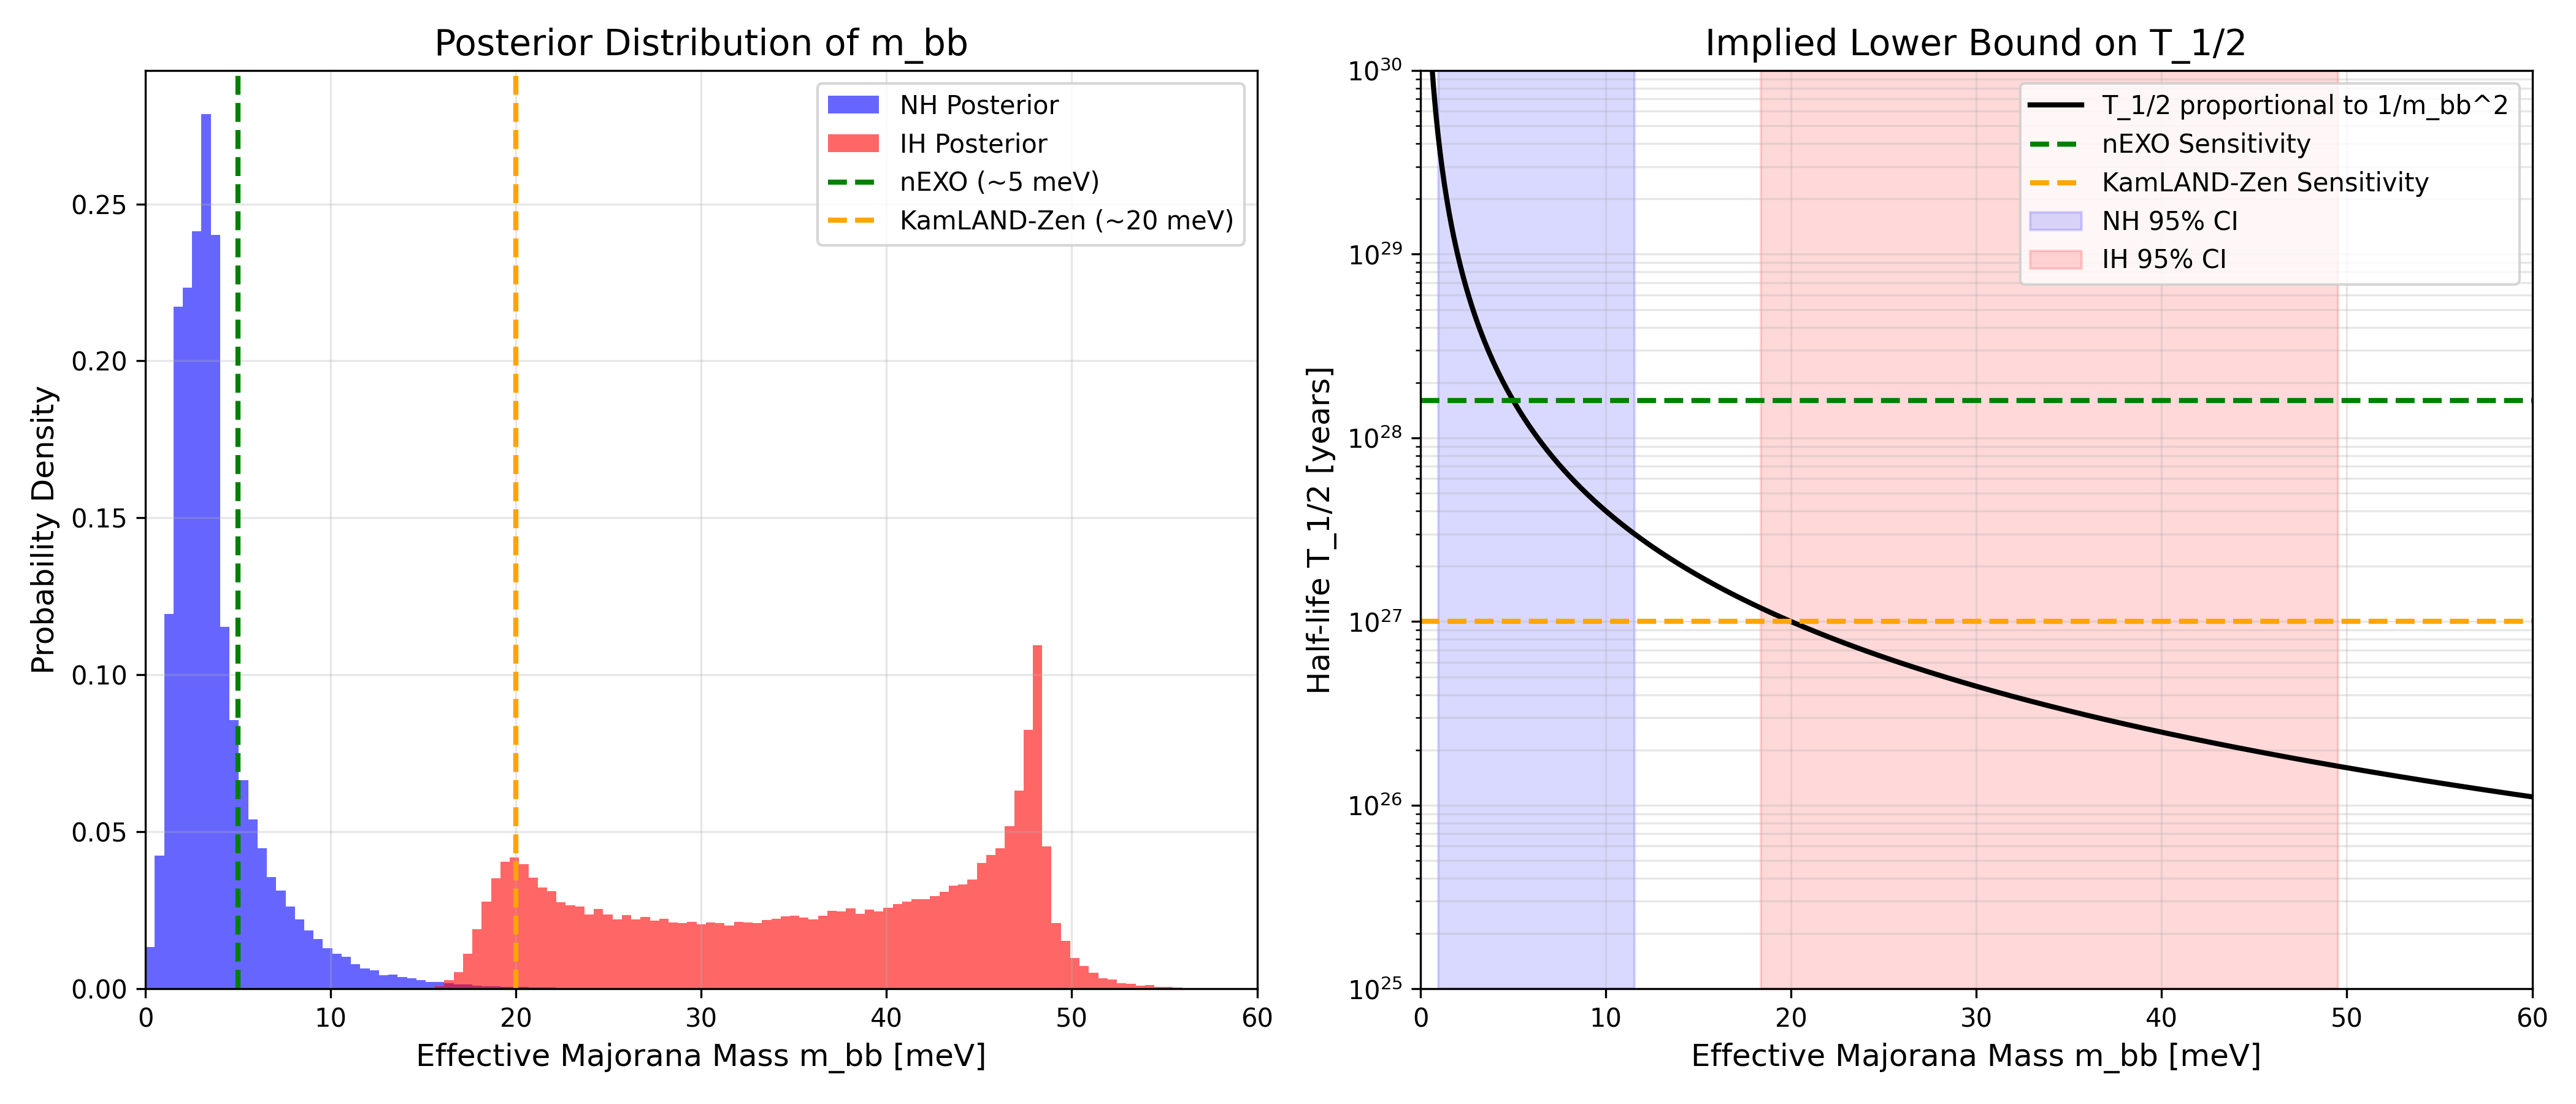
\includegraphics[width=\columnwidth]{../input_files/plots/step_6_mbb_projections_6_20260501_182338.png}
    \caption{Posterior probability distributions for the effective Majorana mass ($m_{\beta\beta}$) for the Normal Hierarchy (NH, blue) and Inverted Hierarchy (IH, red). The left panel shows the NH posterior is concentrated at low values, with a 95\% credible interval of [0.95, 11.55] meV, largely below the projected sensitivity of next-generation experiments like nEXO. Conversely, the IH posterior predicts a much larger signal with a 95\% credible interval of [18.36, 49.51] meV, which would be well within experimental reach. The right panel translates these distributions into the implied lower bound on the neutrinoless double-beta decay half-life ($T_{1/2}$), demonstrating that the NH scenario points towards a half-life likely exceeding $10^{28}$ years, making a non-detection in upcoming experiments the most probable outcome.}
    \label{fig:mbb_projections}
\end{figure}

\subsection{Robustness to the dark energy model}
A critical test of our conclusion is its robustness against extensions to the standard cosmological model. We re-evaluated the Bayesian evidence using a $w_0w_a$CDM model, where a time-varying dark energy equation of state can be degenerate with $\Sigma m_\nu$. In this extended parameter space, the 95\% upper limit on $\Sigma m_\nu$ relaxes to $0.163$\,eV.

As shown in Figure~\ref{fig:bayes_factors_summary}, the Bayes factors decrease as the tension with the IH minimum mass is alleviated. The SJPV prior yields $K_{\text{full}} = 482.1$, maintaining a ``decisive'' classification. The objective HS prior drops to $K_{\text{full}} = 42.6$. While this is a significant reduction from the $\Lambda$CDM baseline ($K_{\text{full}} = 464.6$), a Bayes factor of 42.6 still constitutes ``strong'' evidence for the Normal Hierarchy on the Jeffreys scale. This demonstrates that the statistical preference for the NH remains robust and highly significant even when allowing for a dynamic dark energy equation of state.

\section{Conclusions}
\label{sec:conclusions}
In this work, we have addressed the long-standing question of the neutrino mass hierarchy by performing a rigorous Bayesian model comparison between the Normal Hierarchy (NH) and the Inverted Hierarchy (IH). The determination of the hierarchy is a crucial open problem in particle physics, with direct consequences for theories of mass generation and for the experimental search for neutrinoless double-beta decay. Our analysis leverages the unprecedented statistical power of the latest cosmological data to provide a definitive answer.

Our methodology combines the tightest available cosmological constraint on the sum of neutrino masses, $\Sigma m_\nu$, from the Dark Energy Spectroscopic Instrument (DESI) Data Release 2 with the latest global fit to neutrino oscillation data from NuFIT 6.0. We computed the Bayesian evidence for each hierarchy, quantifying their relative probability with the Bayes factor, $K = P(D|\text{NH}) / P(D|\text{IH})$. To ensure the robustness of our conclusions against prior assumptions, we employed two distinct and well-motivated prior frameworks: a physically-motivated hierarchical (SJPV) prior and a conservative, objective (HS) reference prior.

The results provide decisive evidence in favor of the Normal Hierarchy. The DESI DR2 data, within the standard $\Lambda$CDM model, constrains the total neutrino mass to be $\Sigma m_\nu < 0.0642$\,eV at 95\% confidence. This upper limit lies significantly below the minimum mass required by the Inverted Hierarchy ($\Sigma m_\nu \ge 0.099$\,eV), placing the entire IH parameter space in severe tension with observations. This tension translates into a Bayes factor of $K > 460$ even under the most conservative HS prior, a value that corresponds to ``decisive'' evidence on the Jeffreys scale. The preference remains strong ($K > 40$) even when extending the analysis to a more flexible $w_0w_a$CDM cosmological model, demonstrating that the conclusion is not an artifact of the baseline model assumptions.

From these results, we have learned that the combination of state-of-the-art cosmological and oscillation data is sufficient to resolve the neutrino mass hierarchy. The Normal Hierarchy is not just preferred, but the Inverted Hierarchy is now robustly disfavored. This finding allows us to place strong constraints on the absolute neutrino mass scale, with the posterior for $\Sigma m_\nu$ being tightly peaked around its minimum allowed value of $\sim 0.059$\,eV. A direct and significant consequence of this result is a revised outlook for neutrinoless double-beta decay experiments. Our posterior for the effective Majorana mass, $m_{\beta\beta}$, is suppressed into the few-meV range, with a 95\% credible interval of $[0.95, 11.55]$\,meV. This is in stark contrast to the much larger signal predicted by the now-disfavored Inverted Hierarchy and suggests that the detection of this rare decay will be significantly more challenging than previously anticipated, likely lying beyond the sensitivity of the next generation of experiments. In conclusion, the precision of modern cosmology has provided a pivotal answer to a fundamental question in particle physics, decisively favoring the Normal Neutrino Mass Hierarchy and reshaping the landscape for future searches for new physics.


\bibliography{bibliography}{}
\bibliographystyle{unsrt}

\end{document}
